\chapter{Results and Comparisons} 
\label{ch:results} 
This Chapter contains results and its comparisons from both A-S and ExxonMobil models for all the test cases. More details for the test cases can be find in \chaptername~\ref{ch:testcases}. Summary of the differences between the two models are shown in \tablename~\ref{table_model_difference}.
\begin{table}[!hbt]
\centering
\begin{tabular}{|c|p{1.8in}|p{1.8in}|c|}
\hline 
\tablecolumnheadervlinesone{} & \tablecolumnheadervlinestwo{A-S model} & \tablecolumnheadervlinestwo{ExxonMobil Model} \\
\hline
Motion & Torsional & Torsional + Axial\\                                                              
\hline
Bit model & Constant & Dynamic \\                                                  
\hline
Friction model & Coulomb friction as a jump (see \chaptername~\ref{ch:aarnessshormodel}) & Stribeck  effect: Coulomb + Viscous Friction \\    
\hline
System & PDE & ODE\\                                              
\hline
Solving method. & Forward scheme  & ODE45 Runge Kutta \\   
\hline       
Model approach & Distributed model & Lump Mass Spring \\
\hline      
\end{tabular}
\caption[Summary of the difference between two models]{Summary of the difference between A-S and ExxonMobil models.}\label{table_model_difference}
\end{table}
\section{Test Case 1}
The results for Test Case 1 in each model are depicted in \figurename~\ref{figure_testcase1}. Both models exhibited similar outcomes, revealing a fundamental vibration frequency of 0.440 and 0.427 from A-S model and ExxonMobil model, respecitvley. The maximum bit velocity was at 79 RPM for the A-S model and 81 RPM for the ExxonMobil model. Also, the torque on the top drive was predicted as 1762 lb-ft for the A-S model and 1814 lb-ft for the ExxonMobil model. The comparison between the results from different models are illustrated in \figurename~\ref{figure_testcase1_overlapped}. Although both models exhibited similar frequencies, the minimal phase differences contribute to the observed shift between the two models.
\begin{figure}
  \centering
  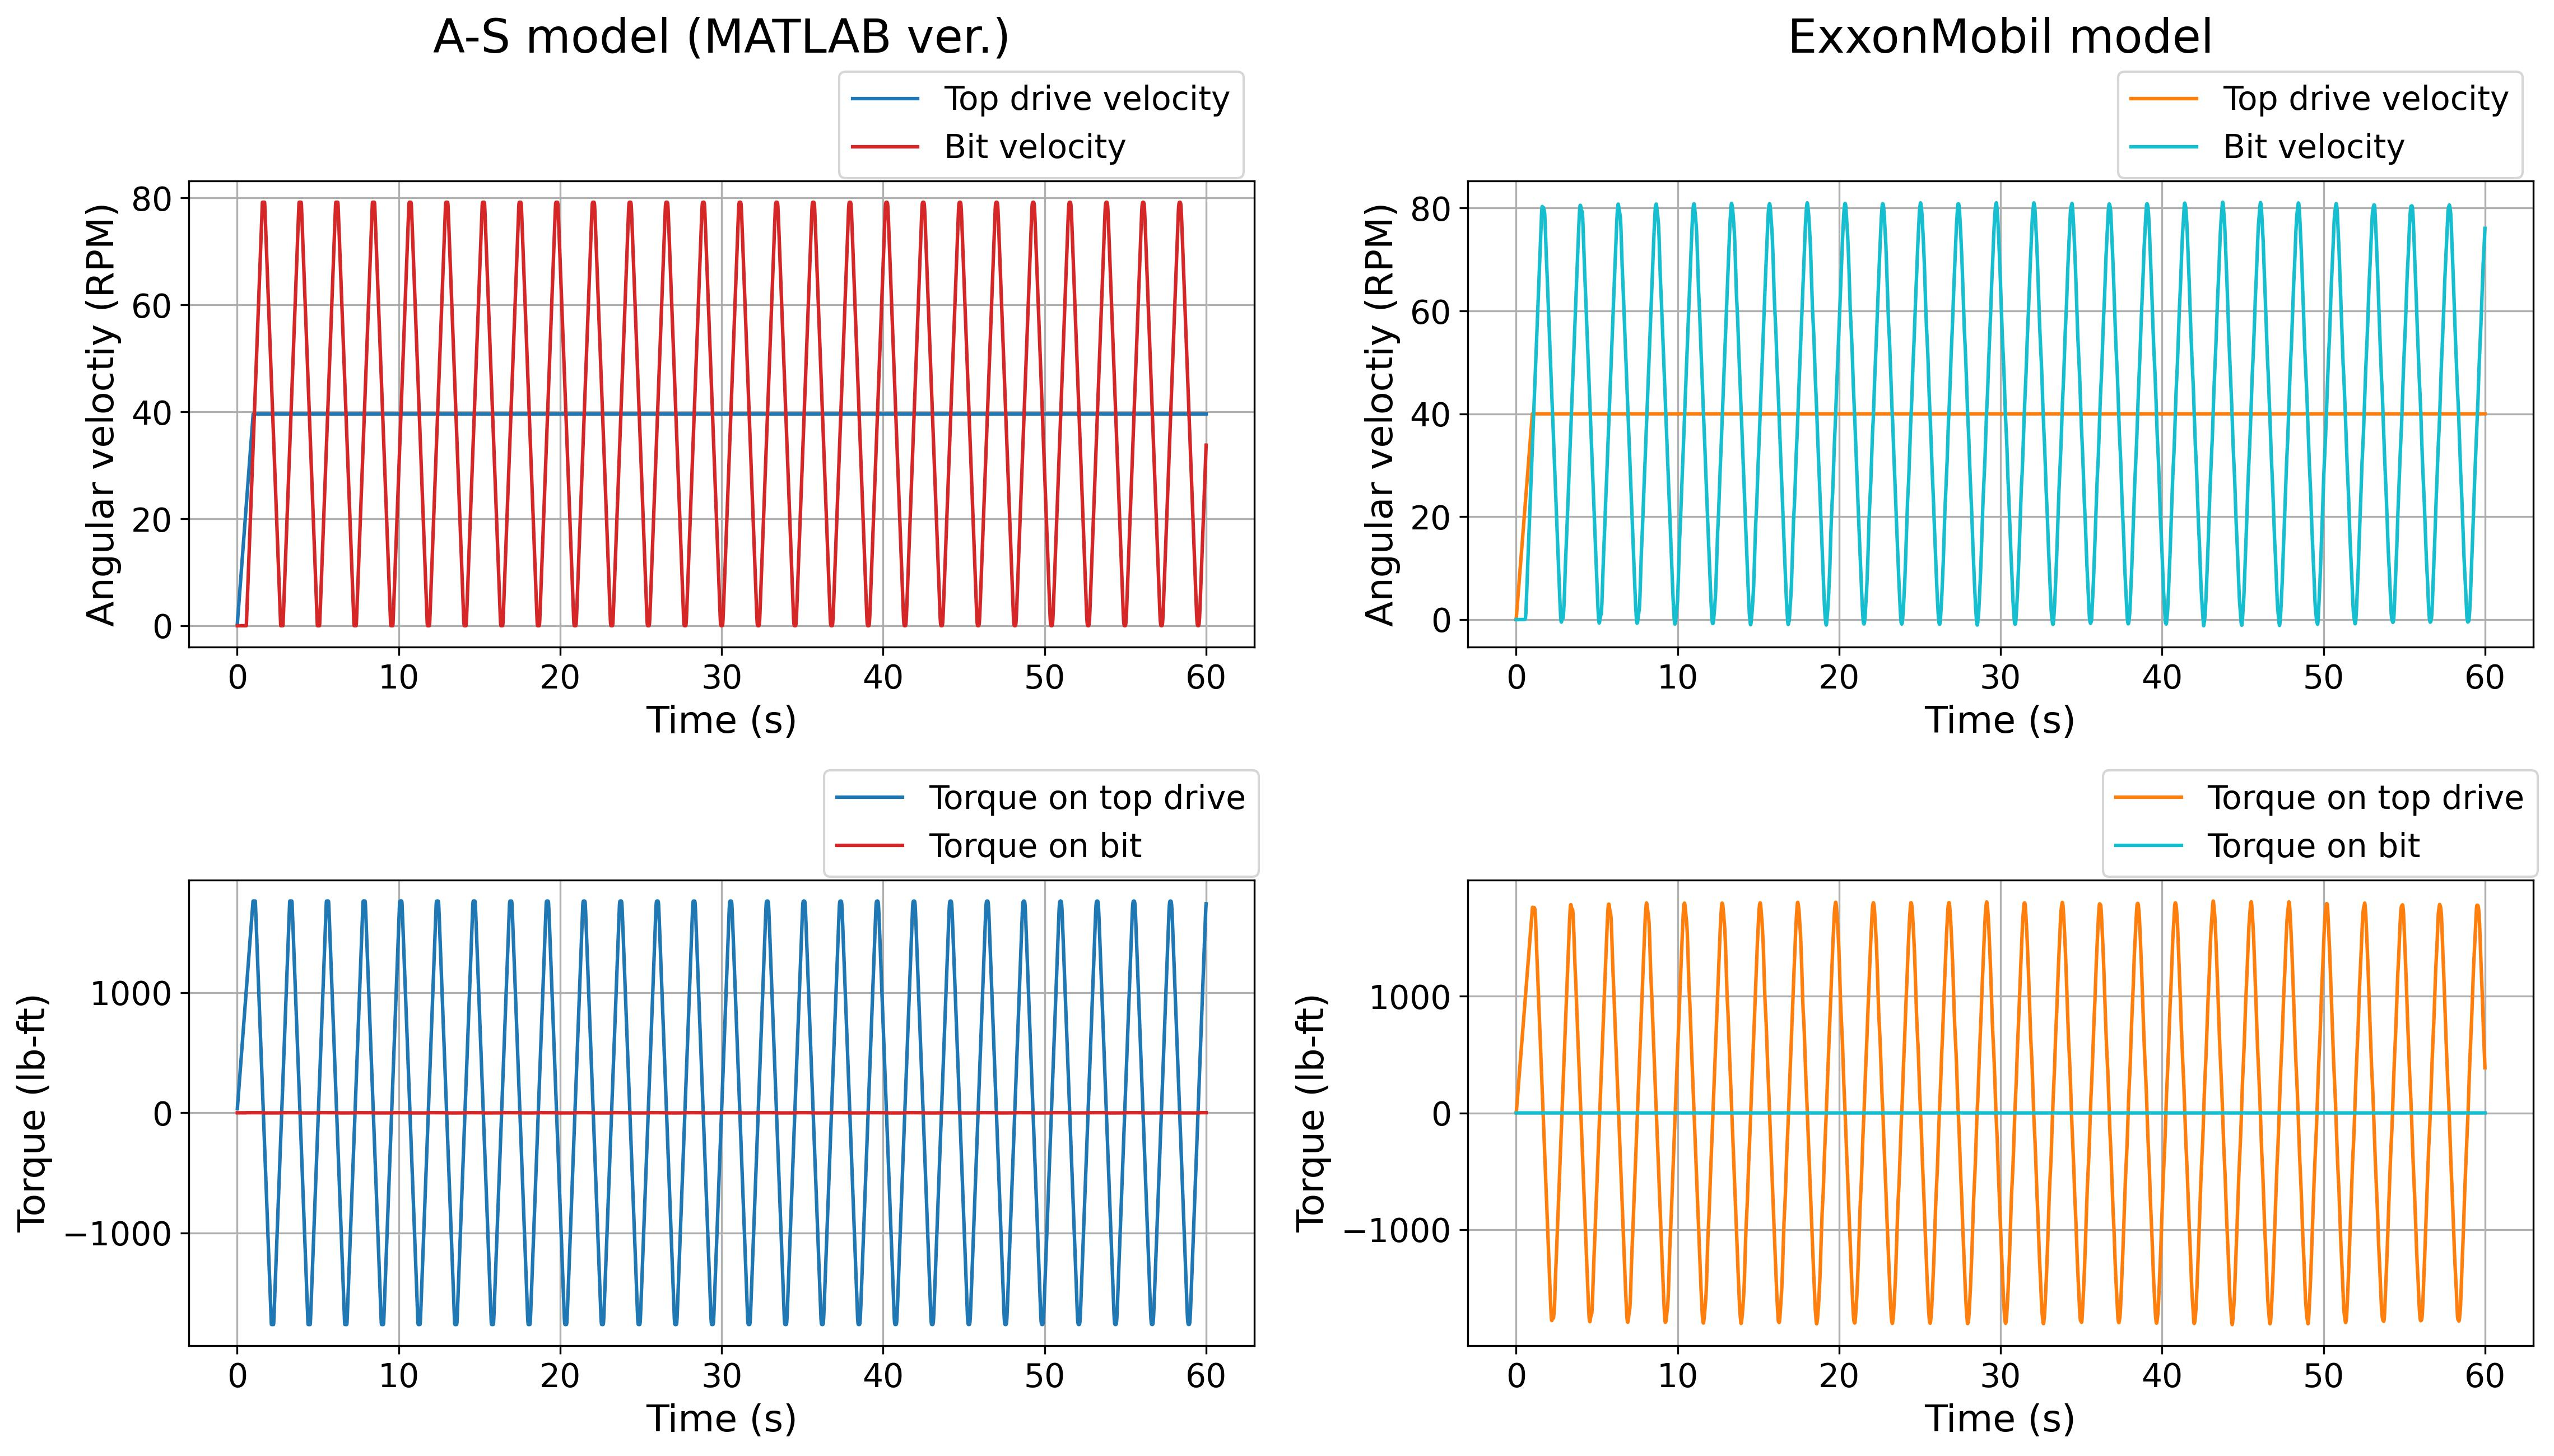
\includegraphics[width=6.5in]{output_figureTestCase1}
  \caption[Results of Test Case 1]{Results of Test Case 1. First and second columns show the results from A-S model (MATLAB ver.) and ExxonMobil model, respectively.}\label{figure_testcase1}
\end{figure}

\begin{figure}
  \centering
  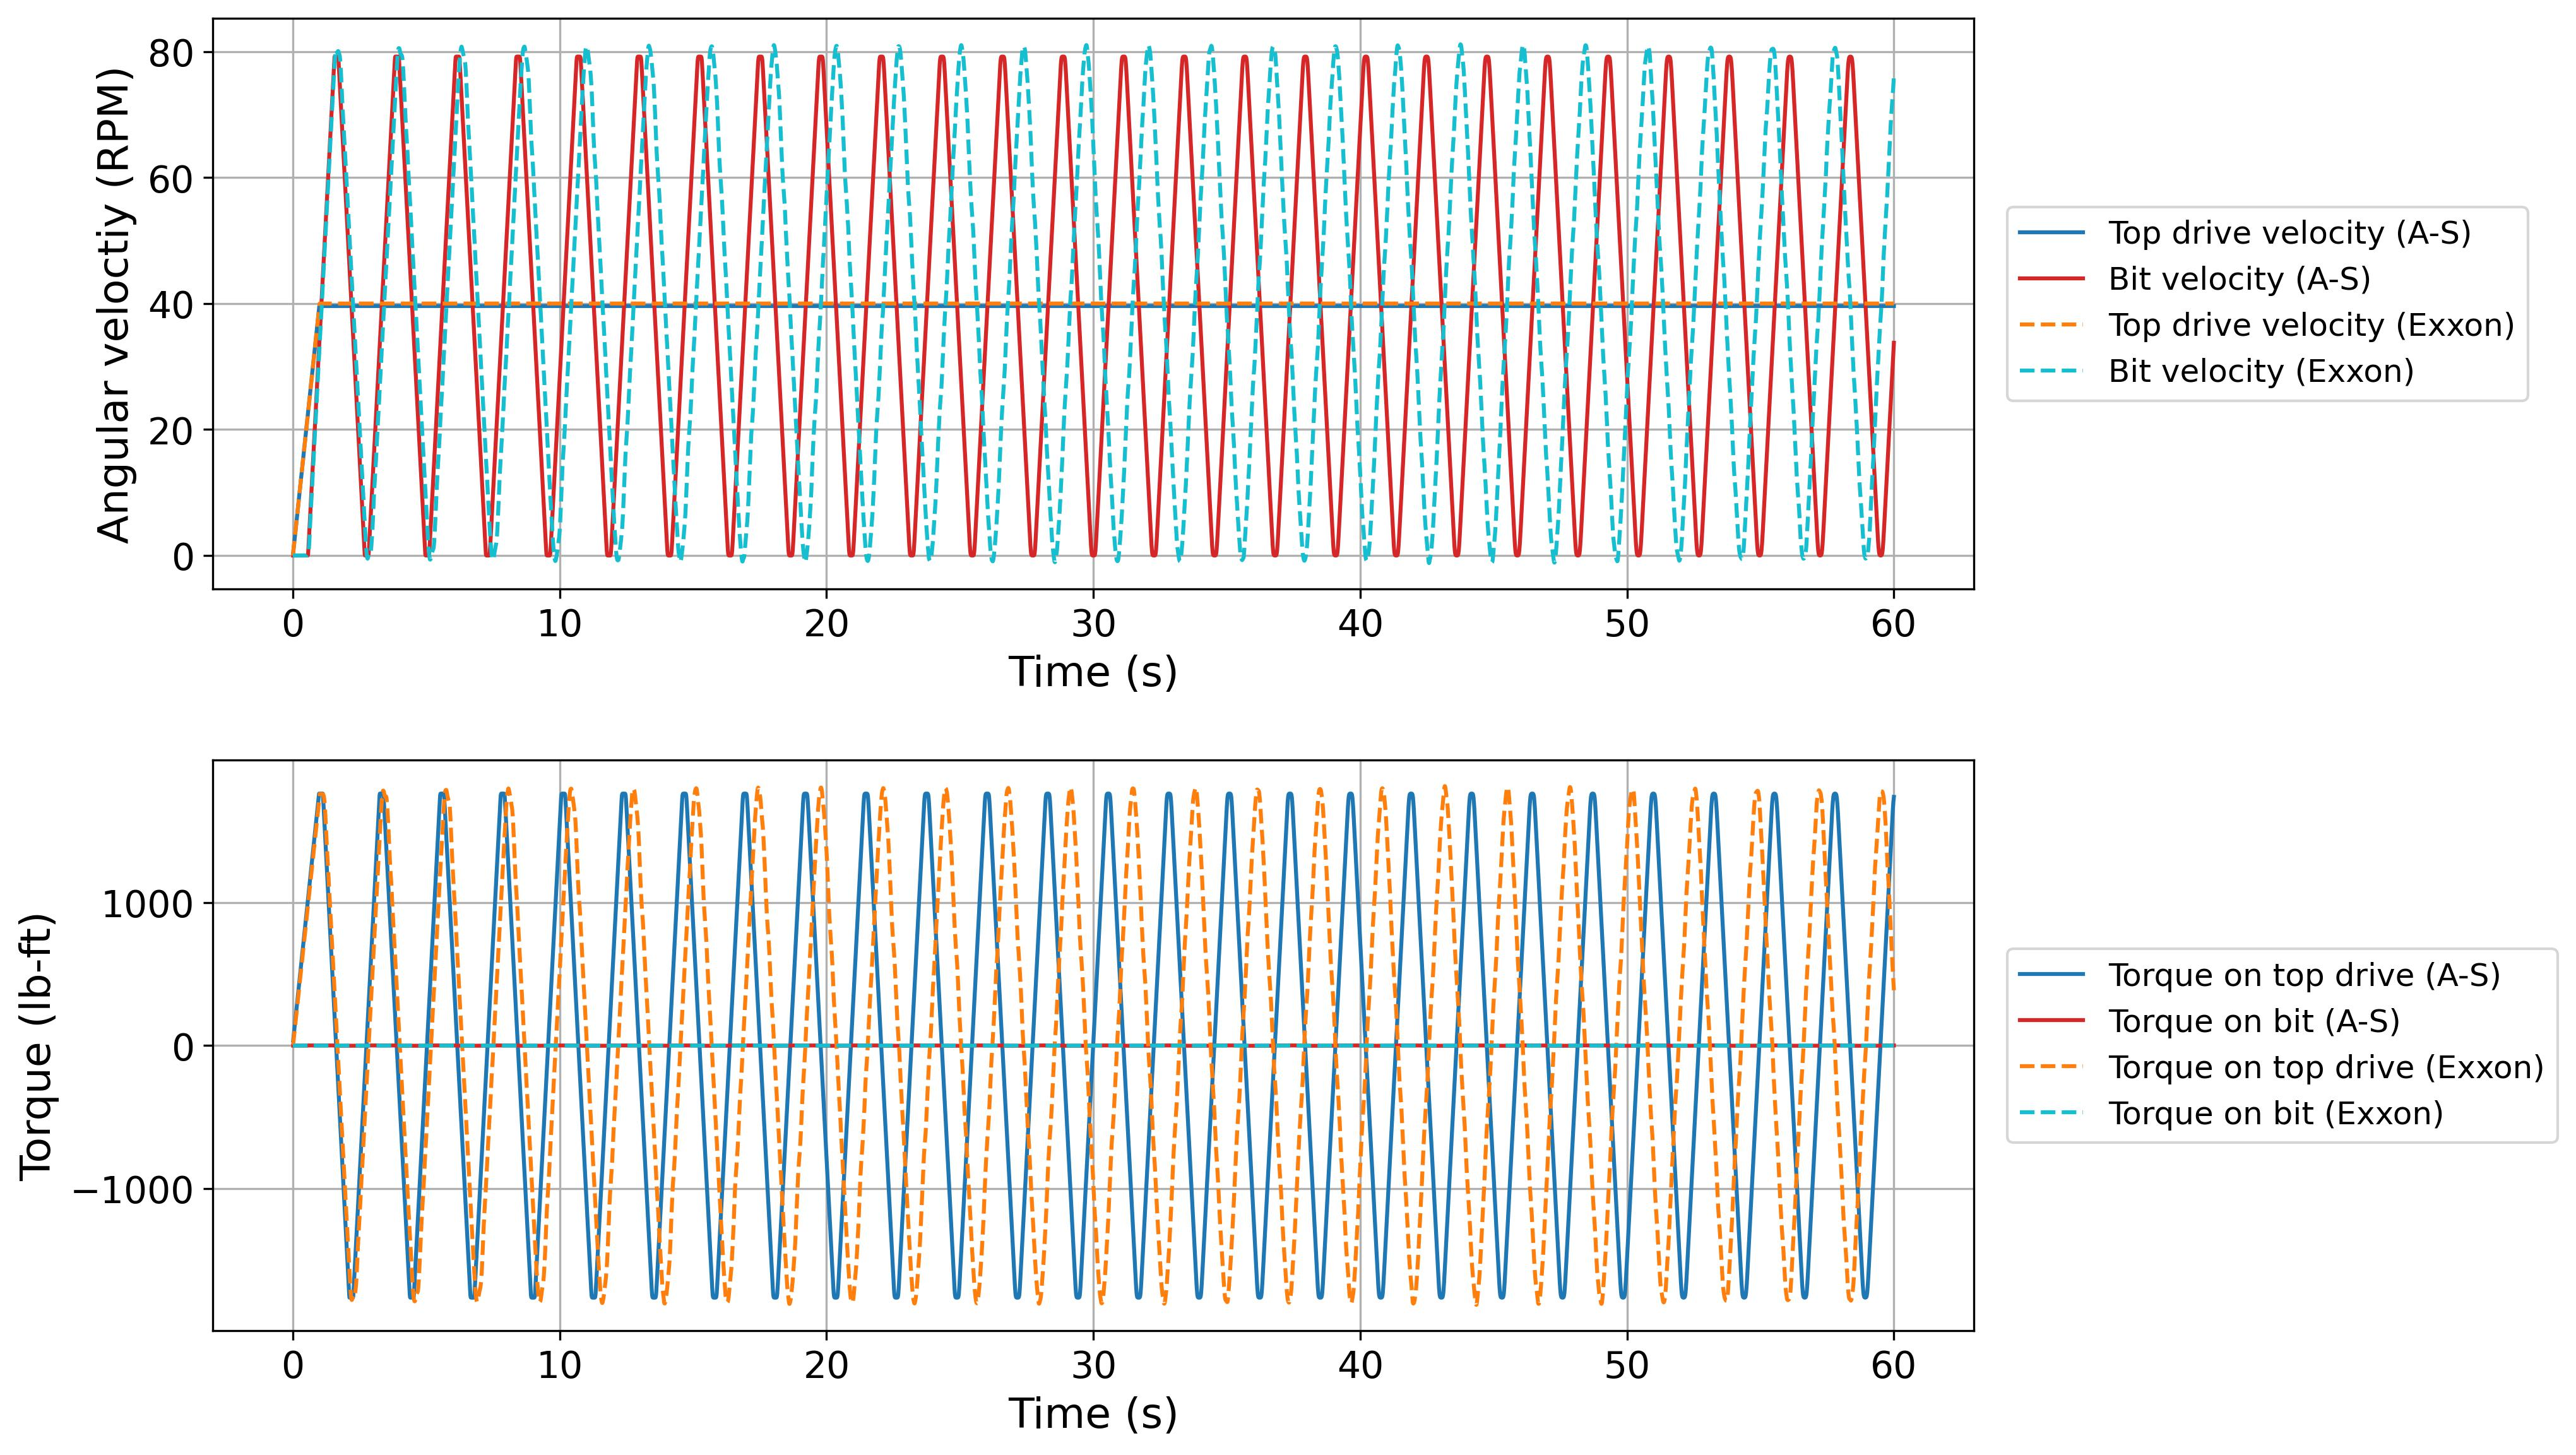
\includegraphics[width=6.5in]{overlapped_figureTestCase1}
  \caption[Comparison of the results for Test Case 1]{Comparison between the results from A-S model (MATLAB ver.) and ExxonMobil model for Test Case 1. The fundamental vibration frequency are 0.440 from A-S model and 0.427 from ExxonMobil model. The difference in frequency is small but the accumulated effect of this differences caused the phase shift during 60 seconds. Overall, both models matched well showing similar amplitude of torque and angular velocity of top drive and bit. }\label{figure_testcase1_overlapped}
\end{figure}

\section{Test Case 2}
\subsection{Test Case 2a}
The results for Test Case 2a from each model are depicted in \figurename~\ref{figure_testcase2_1}. Similar to Test Case 1, both models well matched with fundamental vibration frequencies of 0.283 and 0.272 for A-S model and ExxonMobil model, respectively. The maximum bit velocity was at 78 RPM for the A-S model and 79 RPM for the ExxonMobil model, while the maximum torque on the top drive was predicted as 6643 lb-ft for the A-S model and 6891 lb-ft for the ExxonMobil model. \figurename~\ref{figure_testcase2_1_overlapped} illustrates the comparison of the results from two different models. 
\begin{figure}
  \centering
  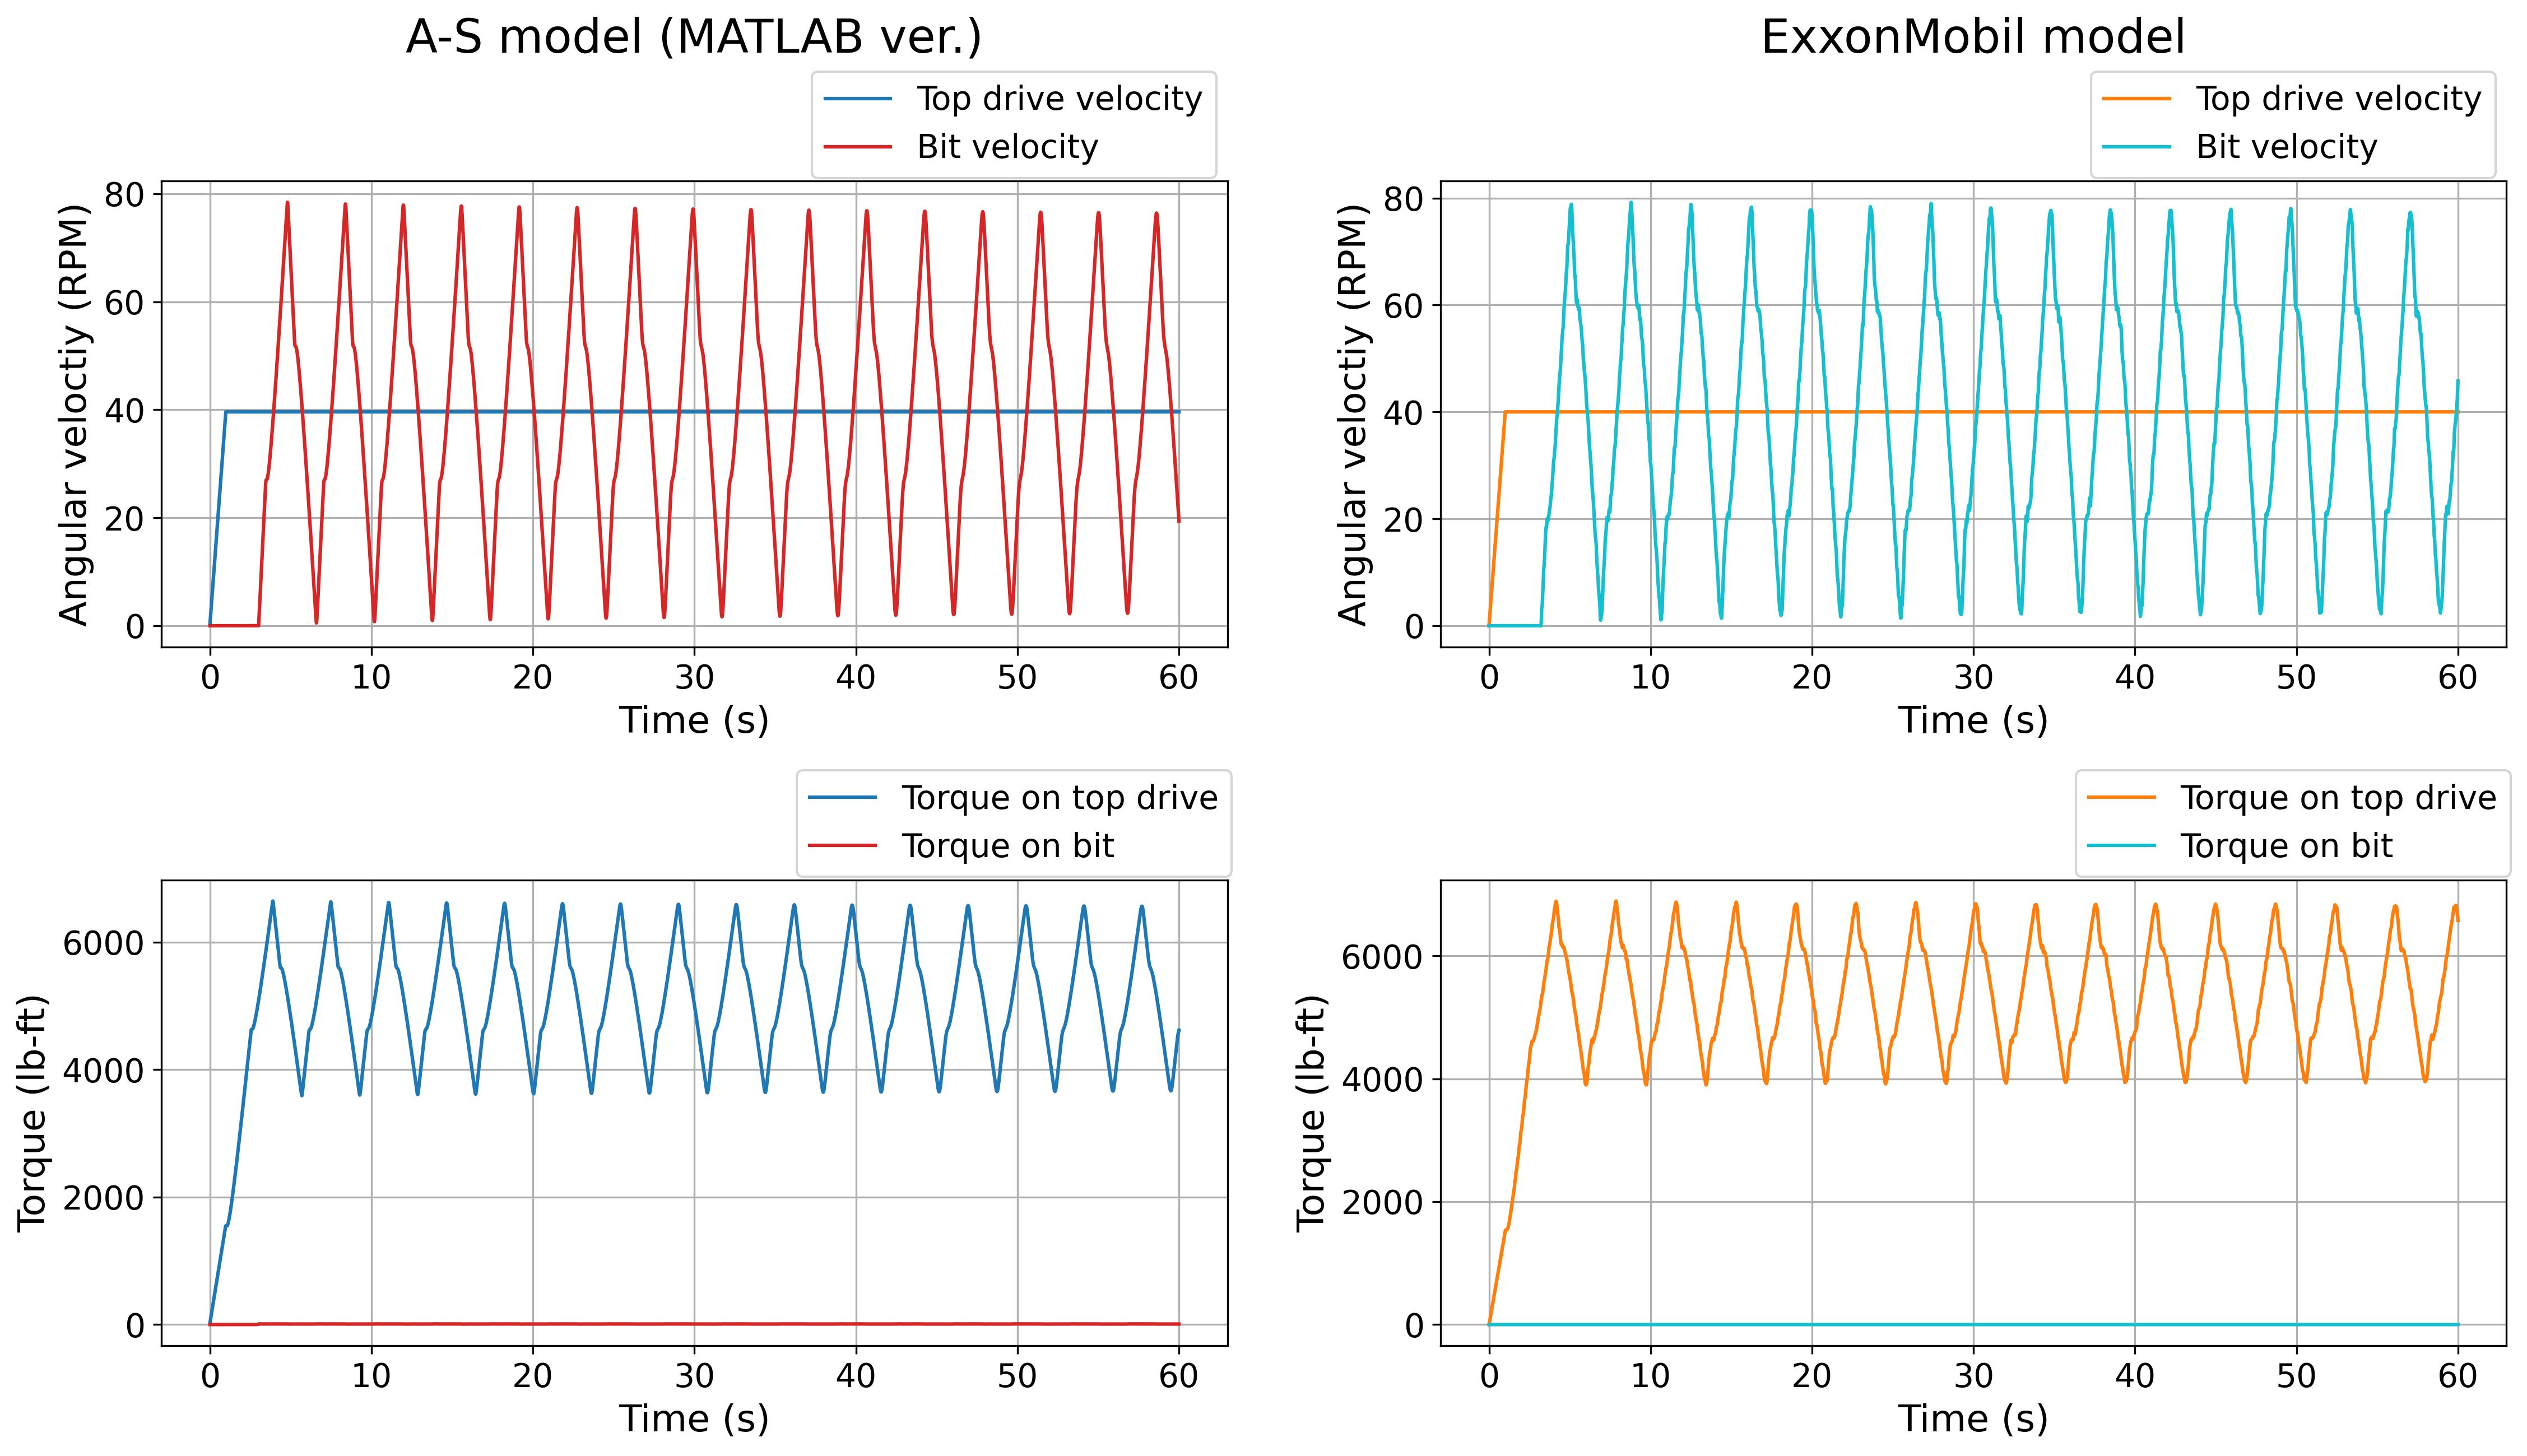
\includegraphics[width=6.5in]{output_figureTestCase2_1}
  \caption[Results of Test Case 2a]{Results of Test Case 2a. First and second columns show the results from A-S model (MATLAB ver.) and ExxonMobil model, respectively.}\label{figure_testcase2_1}
\end{figure}

\begin{figure}
  \centering
  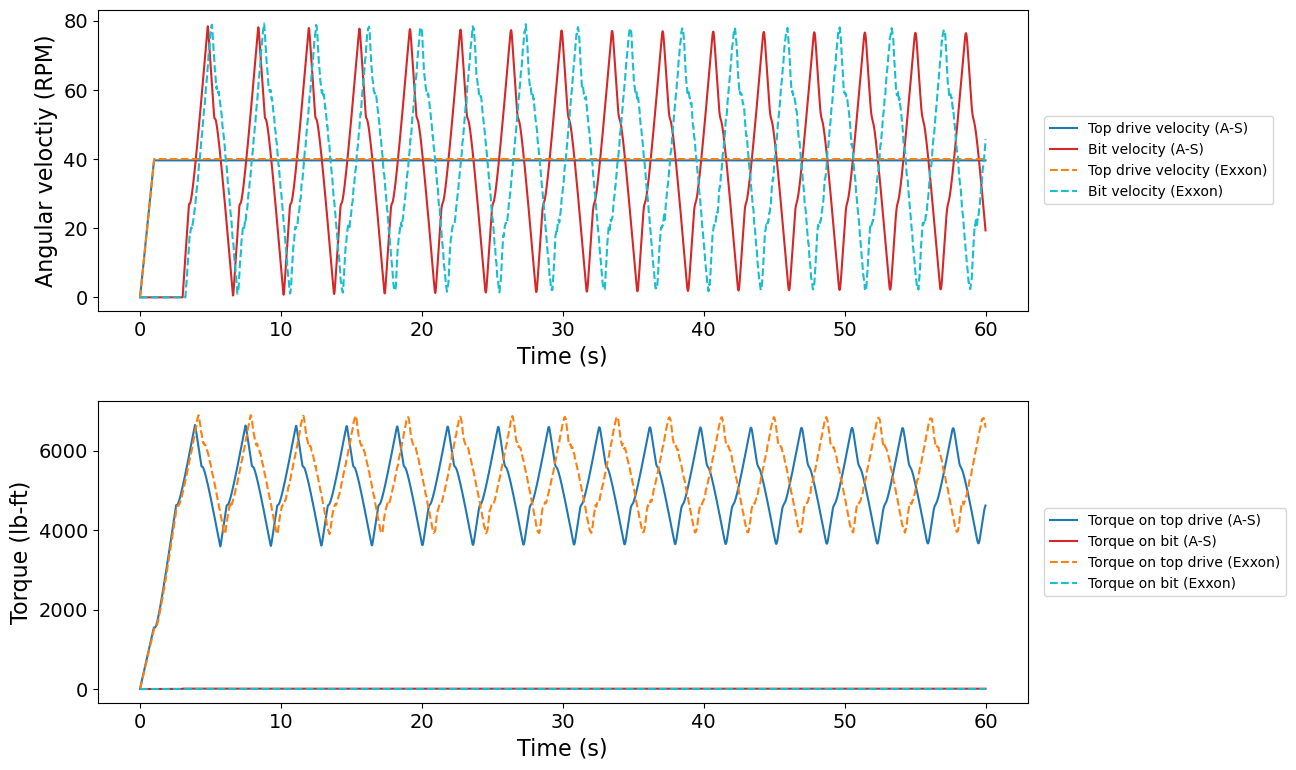
\includegraphics[width=6.5in]{overlapped_figureTestCase2_1}
  \caption[Comparison of the results for Test Case 2a]{Comparison between the results from A-S model (MATLAB ver.) and ExxonMobil model for Test Case 2a. The fundamental vibration frequency are 0.283 from A-S model and 0.272 from ExxonMobil model. The difference in frequency is small but the accumulated effect of this differences caused the phase shift during 60 seconds. Overall, both models matched well showing similar amplitude of torque and angular velocity of top drive and bit.}\label{figure_testcase2_1_overlapped}
\end{figure}


\subsection{Test Case 2b}
The results for Test Case 2b from each model are depicted in \figurename~\ref{figure_testcase2_2}. The stick-slip behavior during drilling was observed in both models. Both models showed transient behavior until 40 seconds and showed almost consistent patterns of vibration after 40 seconds. The time period of the stick phase steadily increased from the beginning and reached about 1.75s for A-S model and 1.78s for ExxonMobil model. This stick-slip event was caused by Coulomb friction from deviated well. This reveals the effect of the dynamic friction factor on the drilling dysfunction since only dynamic friction is reduced to half in Test Case 2b compared to Test Case 2a. Both models showed a spike in bit angular velocity which goes below zero. This has not been investigated yet, but the causation of it can be analyzed in future studies. However, both models showed very similar responses, especially the transient duration (before 40s) even showed very similar responses between the two models.

The fundamental frequencies of the vibration were 0.280 and 0.269 for A-S model and ExxonMobil model, respectively, which are almost the same as Test Case 2a. The maximum bit velocity was at 107 RPM for the A-S model and 116 RPM for the ExxonMobil model. the maximum torque on the top drive was predicted as 5185 lb-ft for the A-S model and 5540 lb-ft for the ExxonMobil model, where the maximum values occurred at the first cycle. \figurename~\ref{figure_testcase2_2_overlapped} illustrates the comparison of the results from two different models during 60 seconds of modeling. Relatively similar behavior can be seen from the comparison, and also the effect of the phase shift was observed.

\begin{figure}
  \centering
  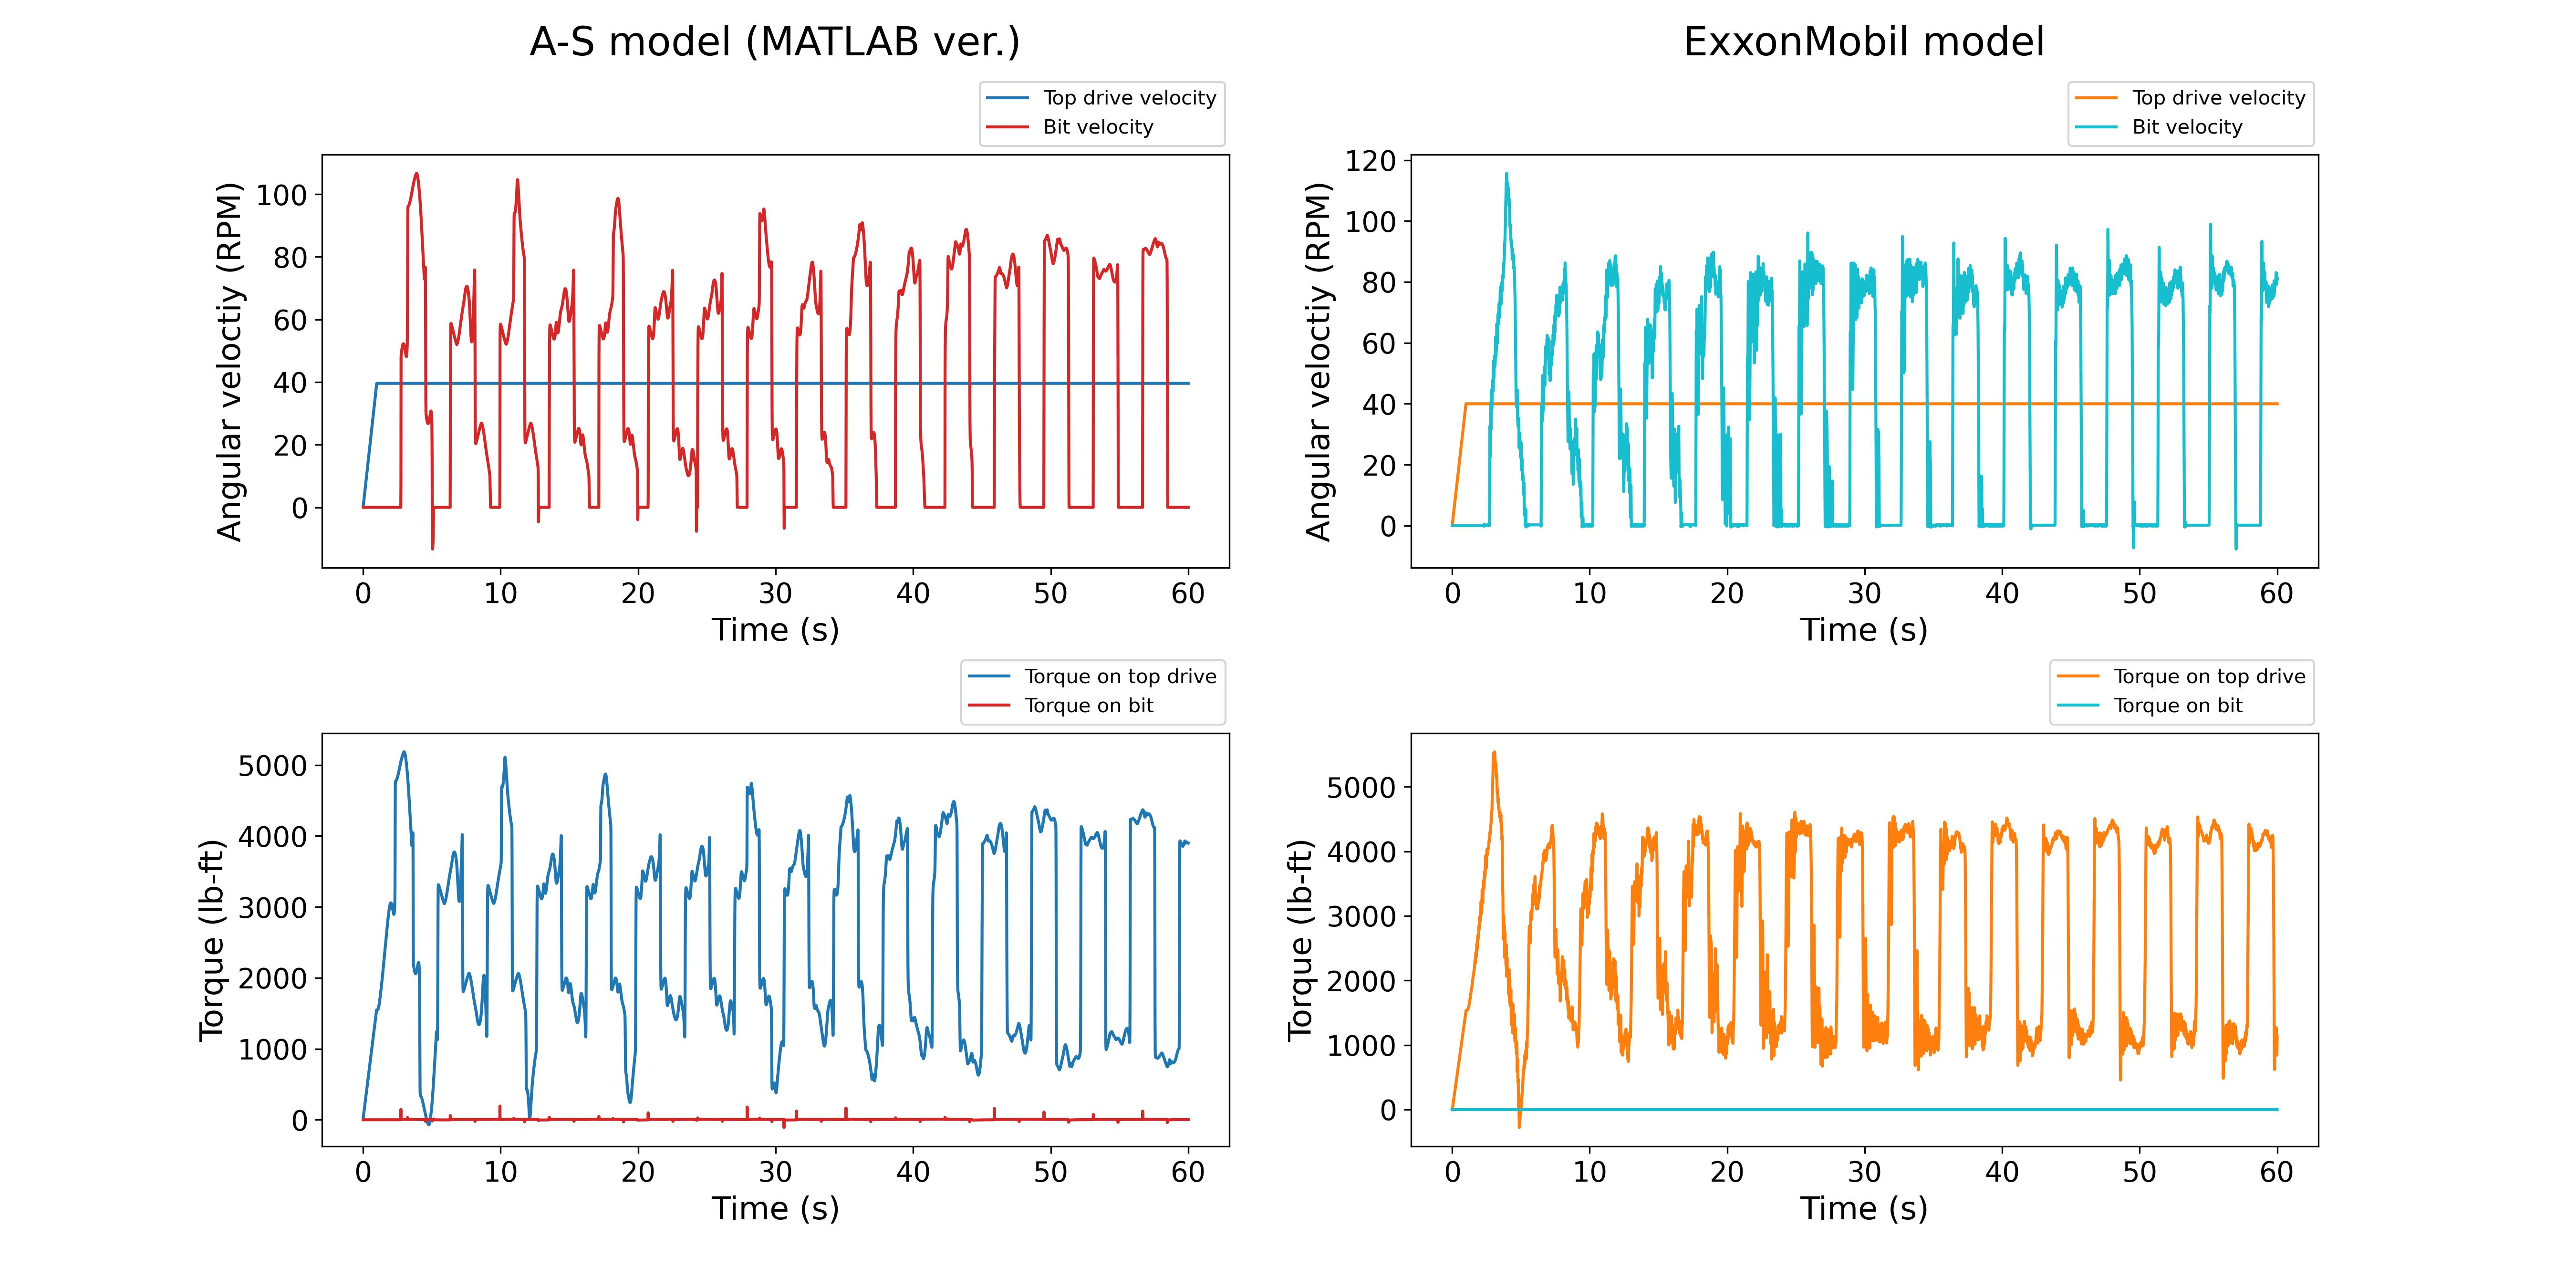
\includegraphics[width=6.5in]{output_figureTestCase2_2}
  \caption[Results of Test Case 2b]{Results of Test Case 2b. First and second columns show the results from A-S model (MATLAB ver.) and ExxonMobil model, respectively.}\label{figure_testcase2_2}
\end{figure}

\begin{figure}
  \centering
  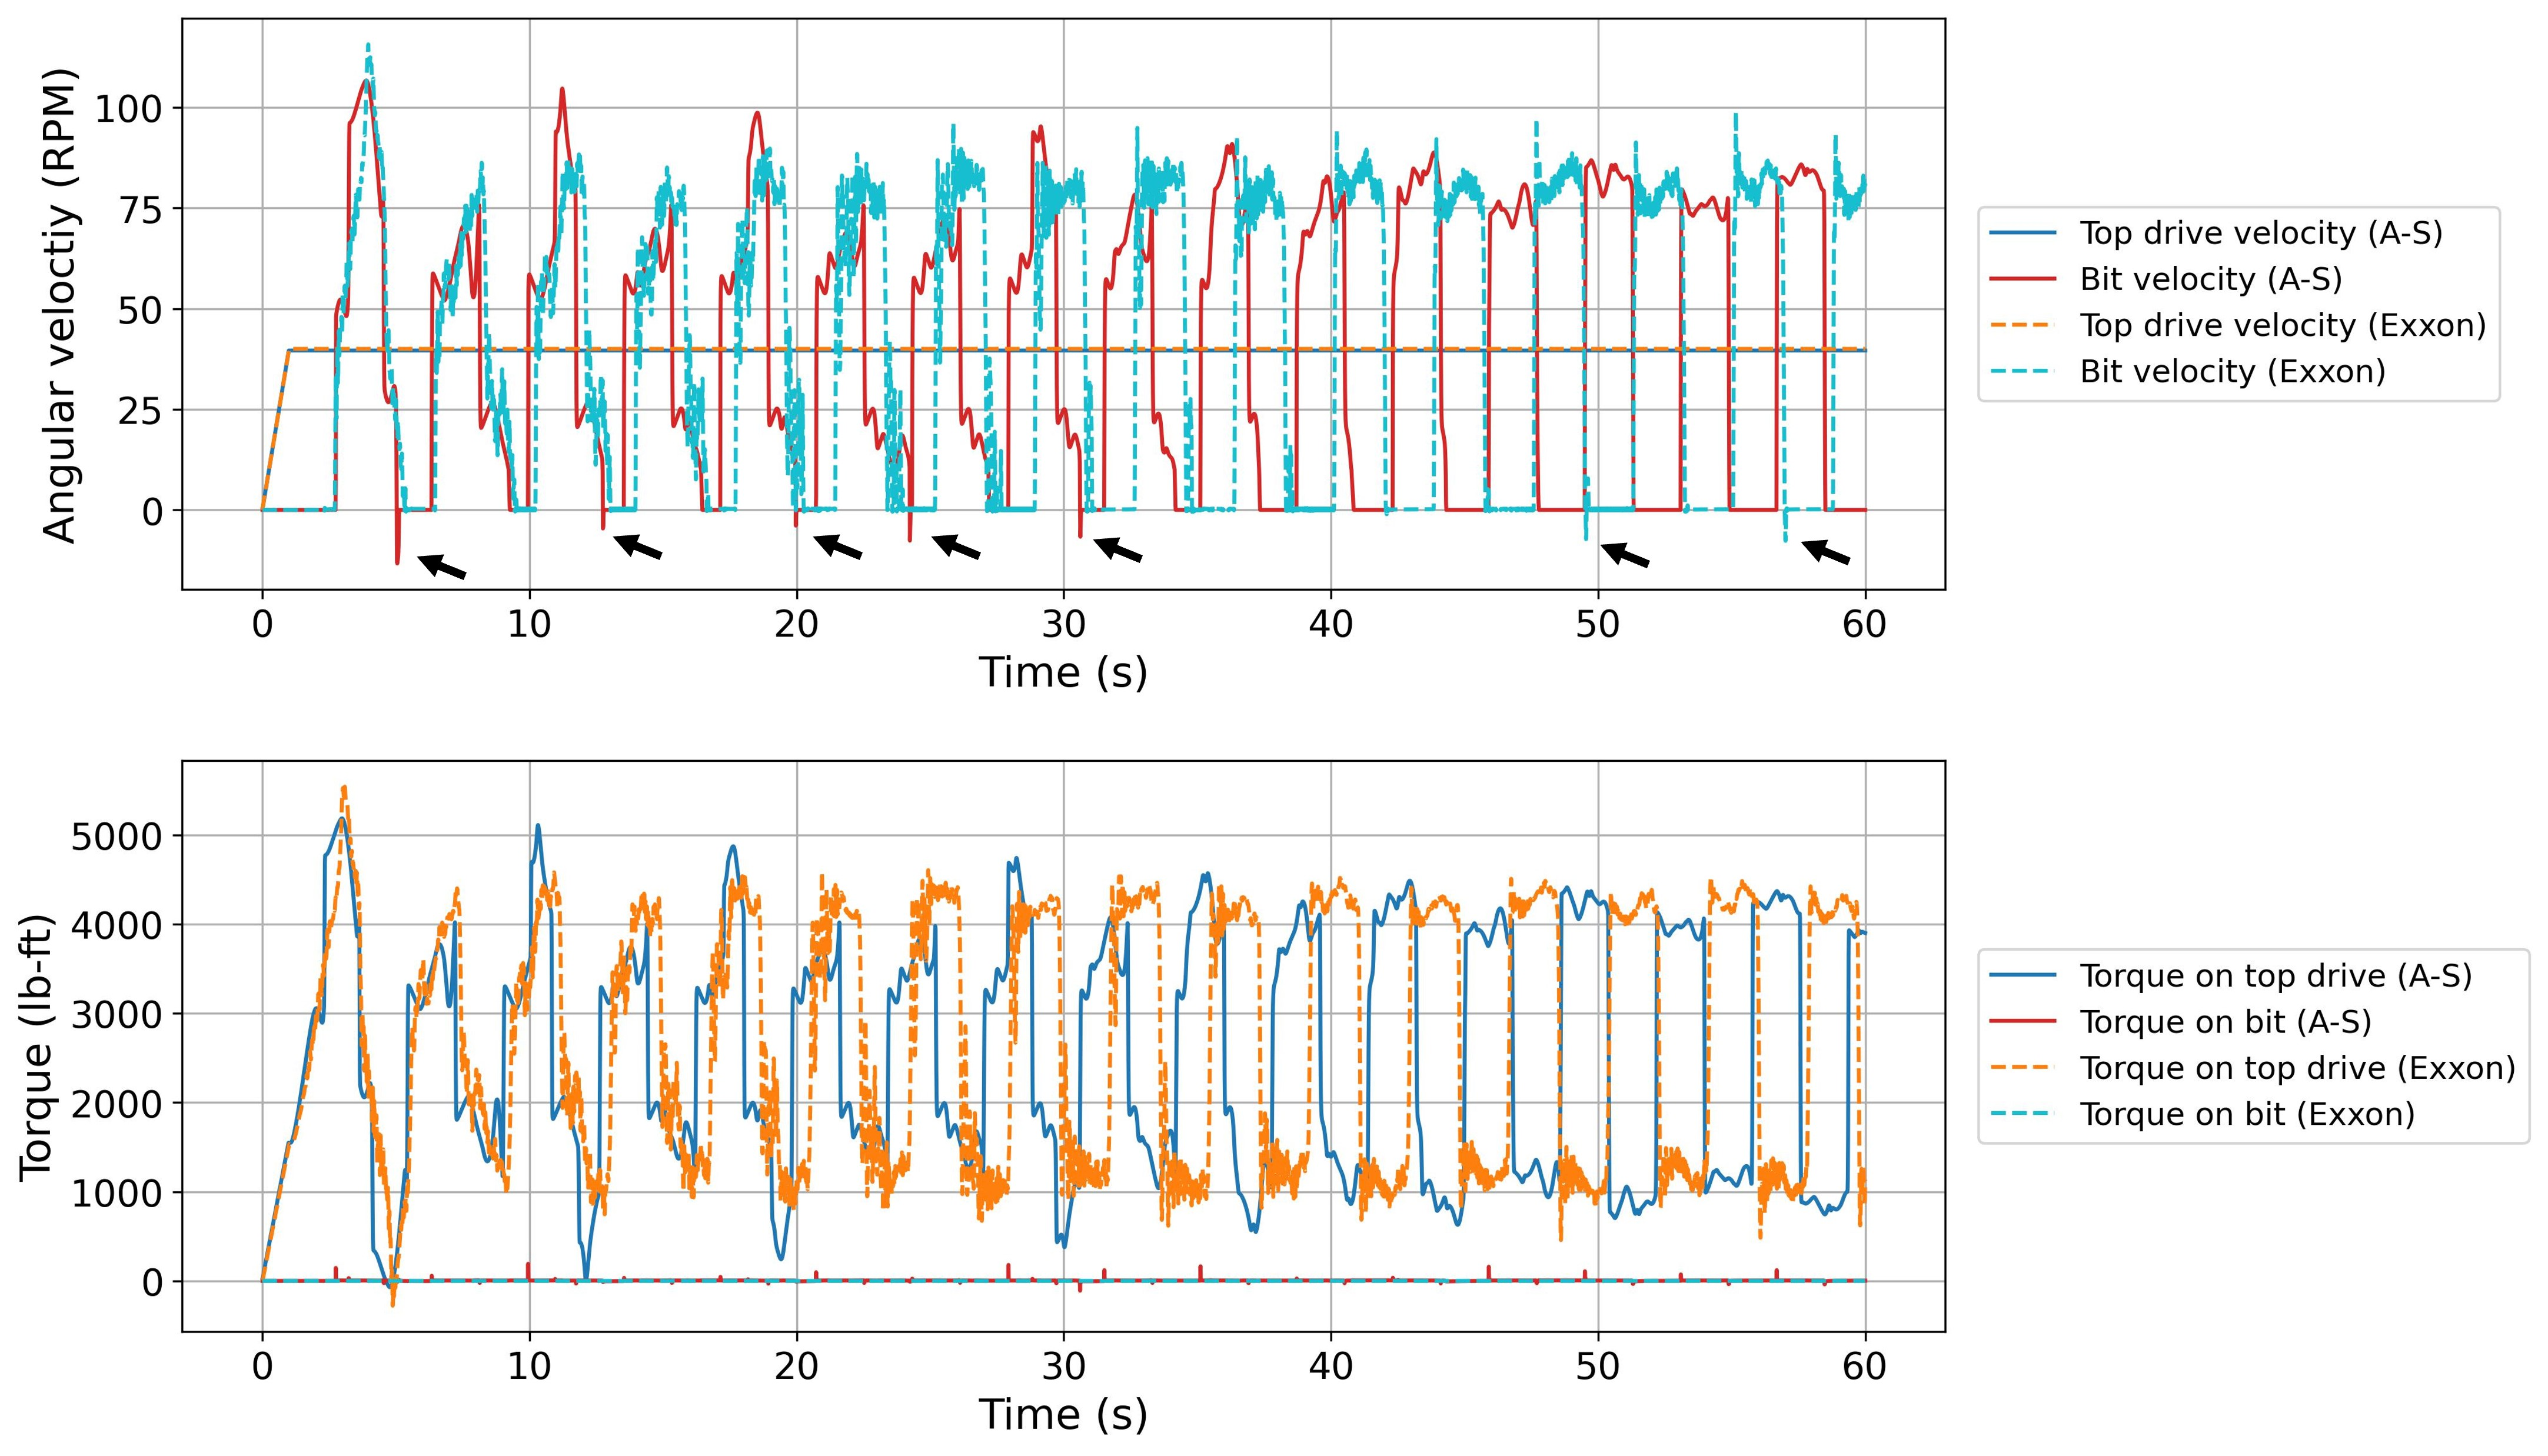
\includegraphics[width=6.5in]{overlapped_figureTestCase2_2_arrow}
  \caption[Comparison of the results for Test Case 2b]{Comparison between the results from A-S model (MATLAB ver.) and ExxonMobil model for Test Case 2b. The fundamental vibration frequency are 0.280 from A-S model and 0.269 from ExxonMobil model. The difference in frequency is small, but the accumulated effect of these differences caused the phase shift during 60 seconds. Overall, both models matched well. Especially the transient phase (before 40s) showed similar vibration patterns for both models. Both models predicted a similar stick time of about 1.6-1.8 seconds during the steady phase (after 40s). The spikes in bit angular velocity ($<$ 0) were observed from both models, which are pointed out by black arrows.}\label{figure_testcase2_2_overlapped}
\end{figure}

\section{Test Case 3}
Test Case 3 shows the effect of BHA components in vertical well. The results show similarities with Test Case 1, but fluctuations in the peak values of the vibration for both bit angular velocity and top drive torque were observed. Specifically, the peak value decreases until 80 seconds and then starts to increase again, ultimately reaching the same value as the beginning at 120 seconds. Figure \ref{figure_testcase3} and Figure \ref{figure_testcase3_overlapped} illustrate the results for each model and comparisons for Test Case 3. \ref{figure_testcase3_overlapped} shows the simulation results for 120 seconds to clearly show the change in the peak values.

Compared to Test Case 1 (without BHA components), the fundamental vibration frequencies in Test Case 3 were slightly decreased, which are 0.420 Hz for the A-S model and 0.408 Hz for the ExxonMobil model. Conversely, the bit velocity and torque on the top drive increased compared to Test Case 3. The maximum bit velocity was 80 RPM for the A-S model and 81 RPM for the ExxonMobil model, while the torque on the top drive was predicted as 1844 lb-ft for the A-S model and 1841 lb-ft for the ExxonMobil model. 

\begin{figure}
  \centering
  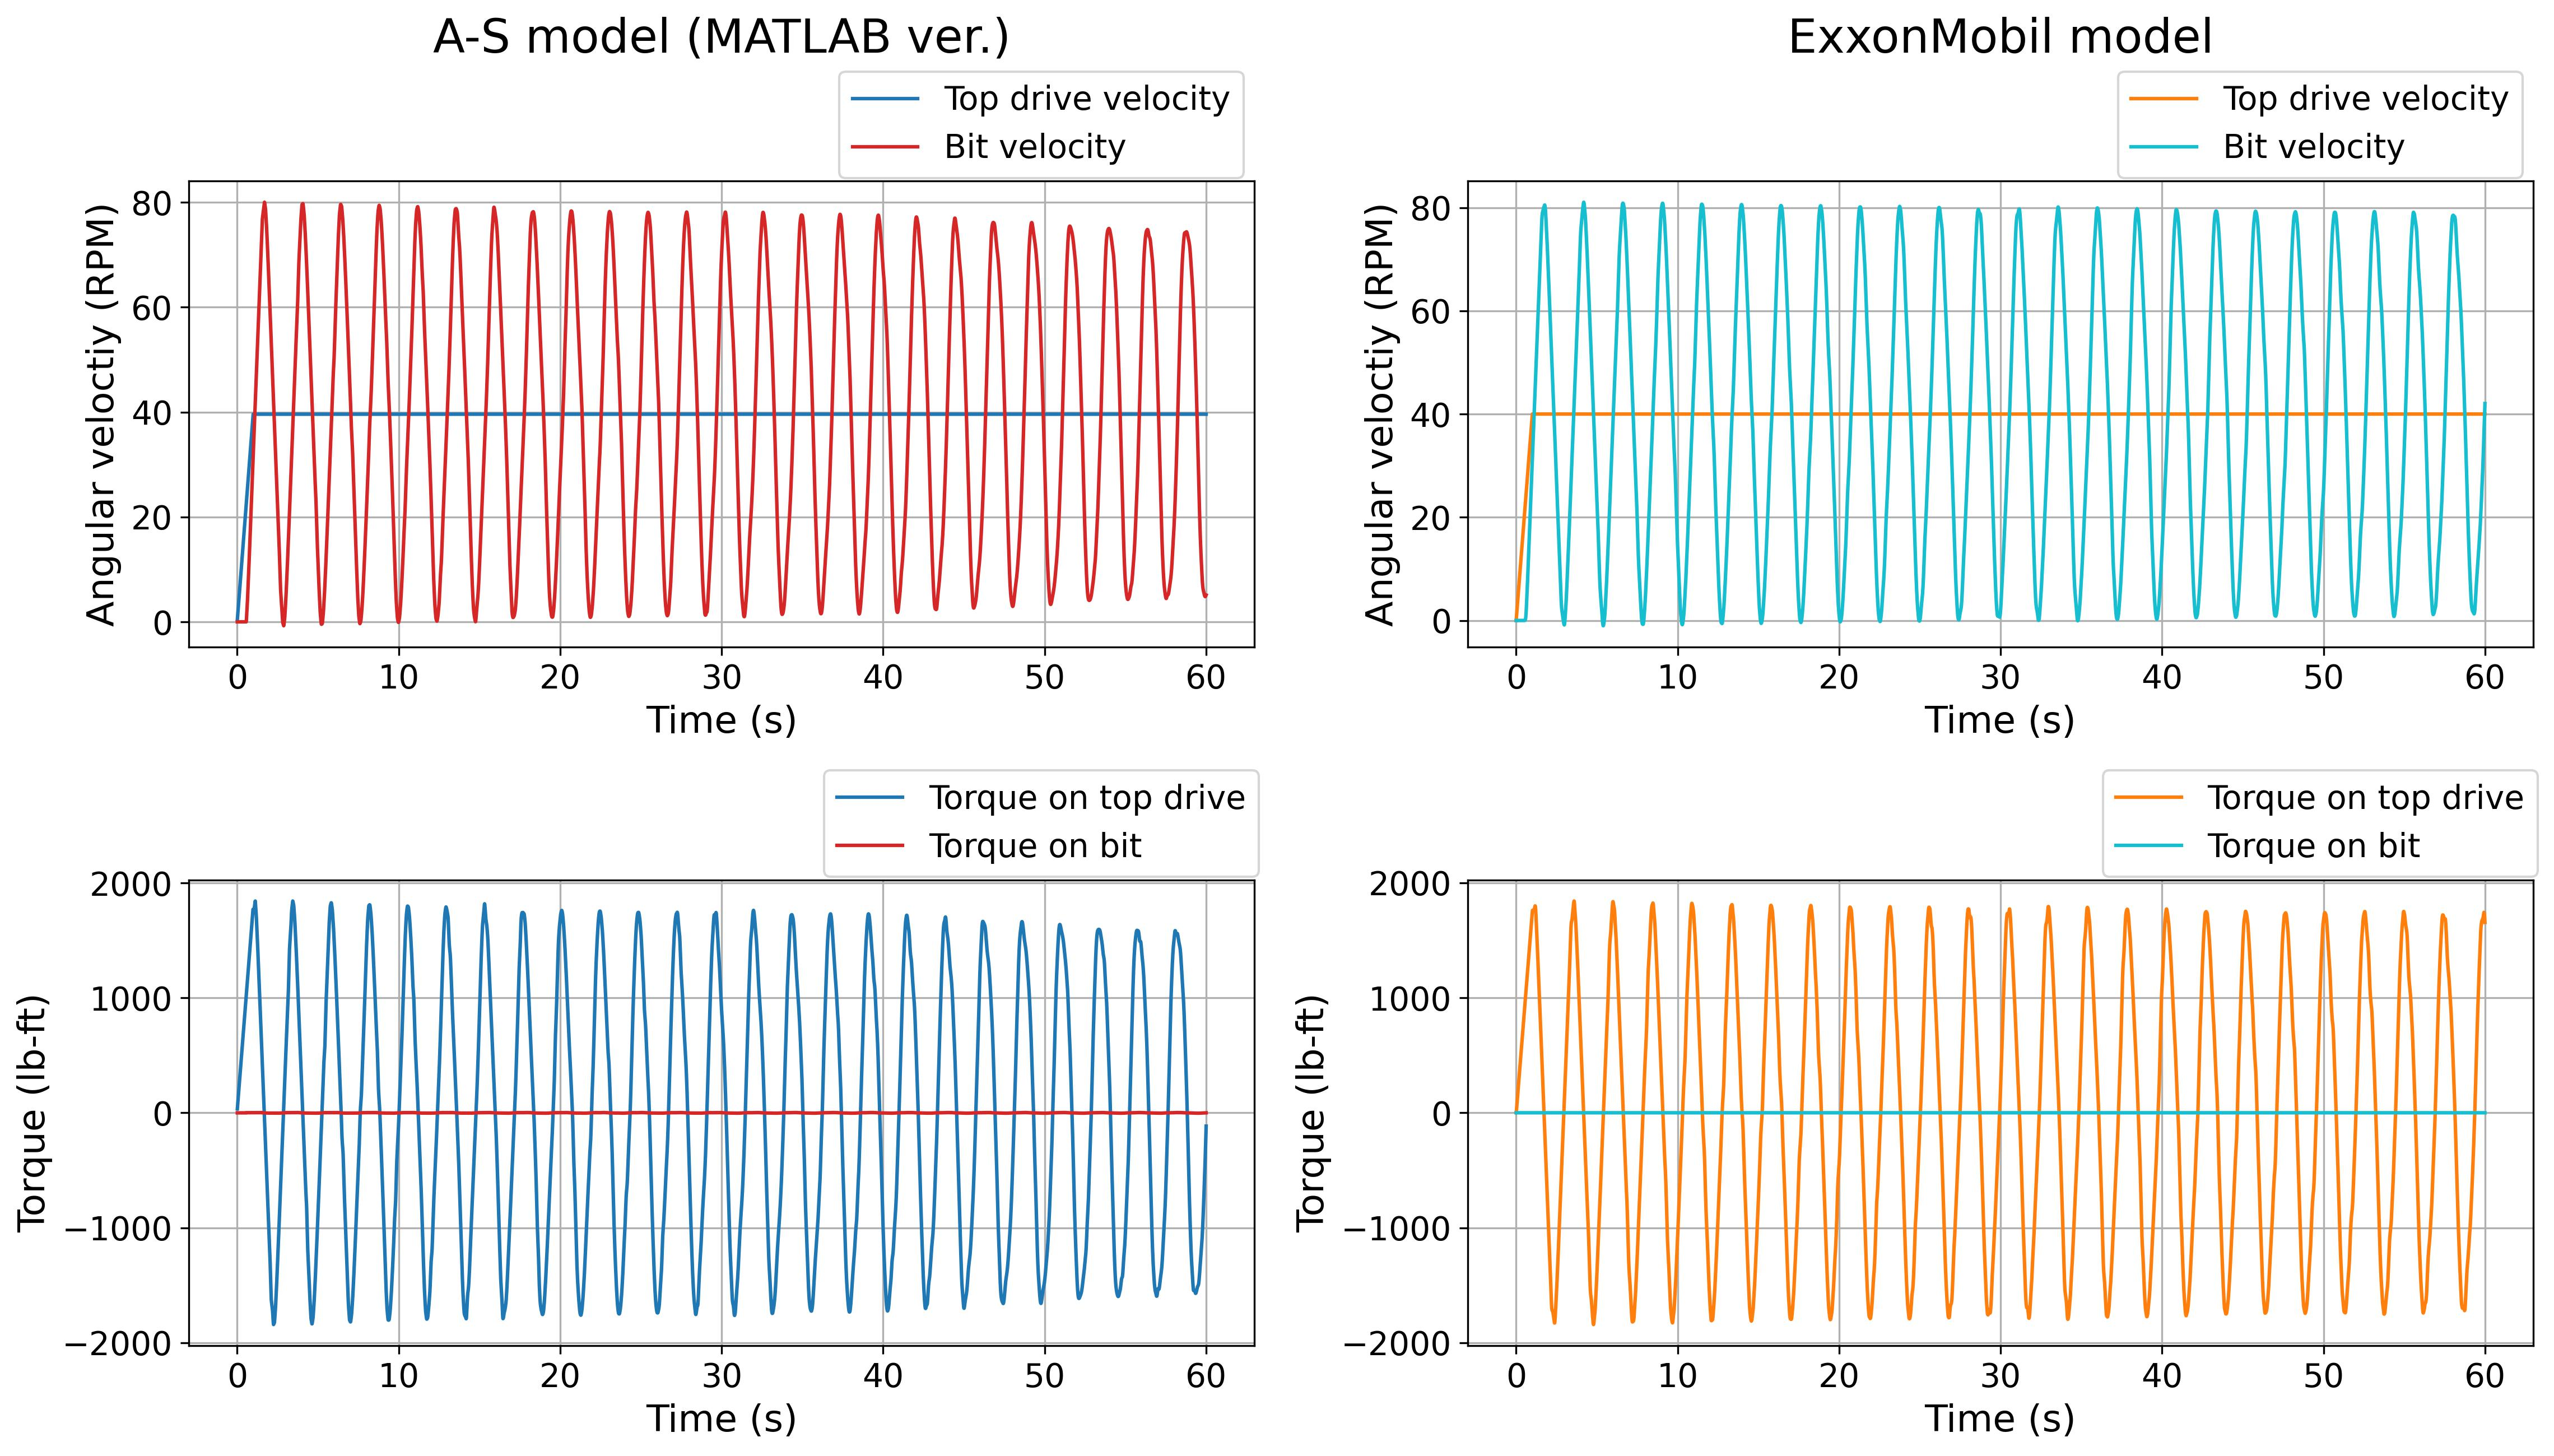
\includegraphics[width=6.5in]{output_figureTestCase3}
  \caption[Results of Test Case 3]{Results of Test Case 3. First and second columns show the results from A-S model (MATLAB ver.) and ExxonMobil model, respectively.}\label{figure_testcase3}
\end{figure}
\begin{figure}
  \centering
  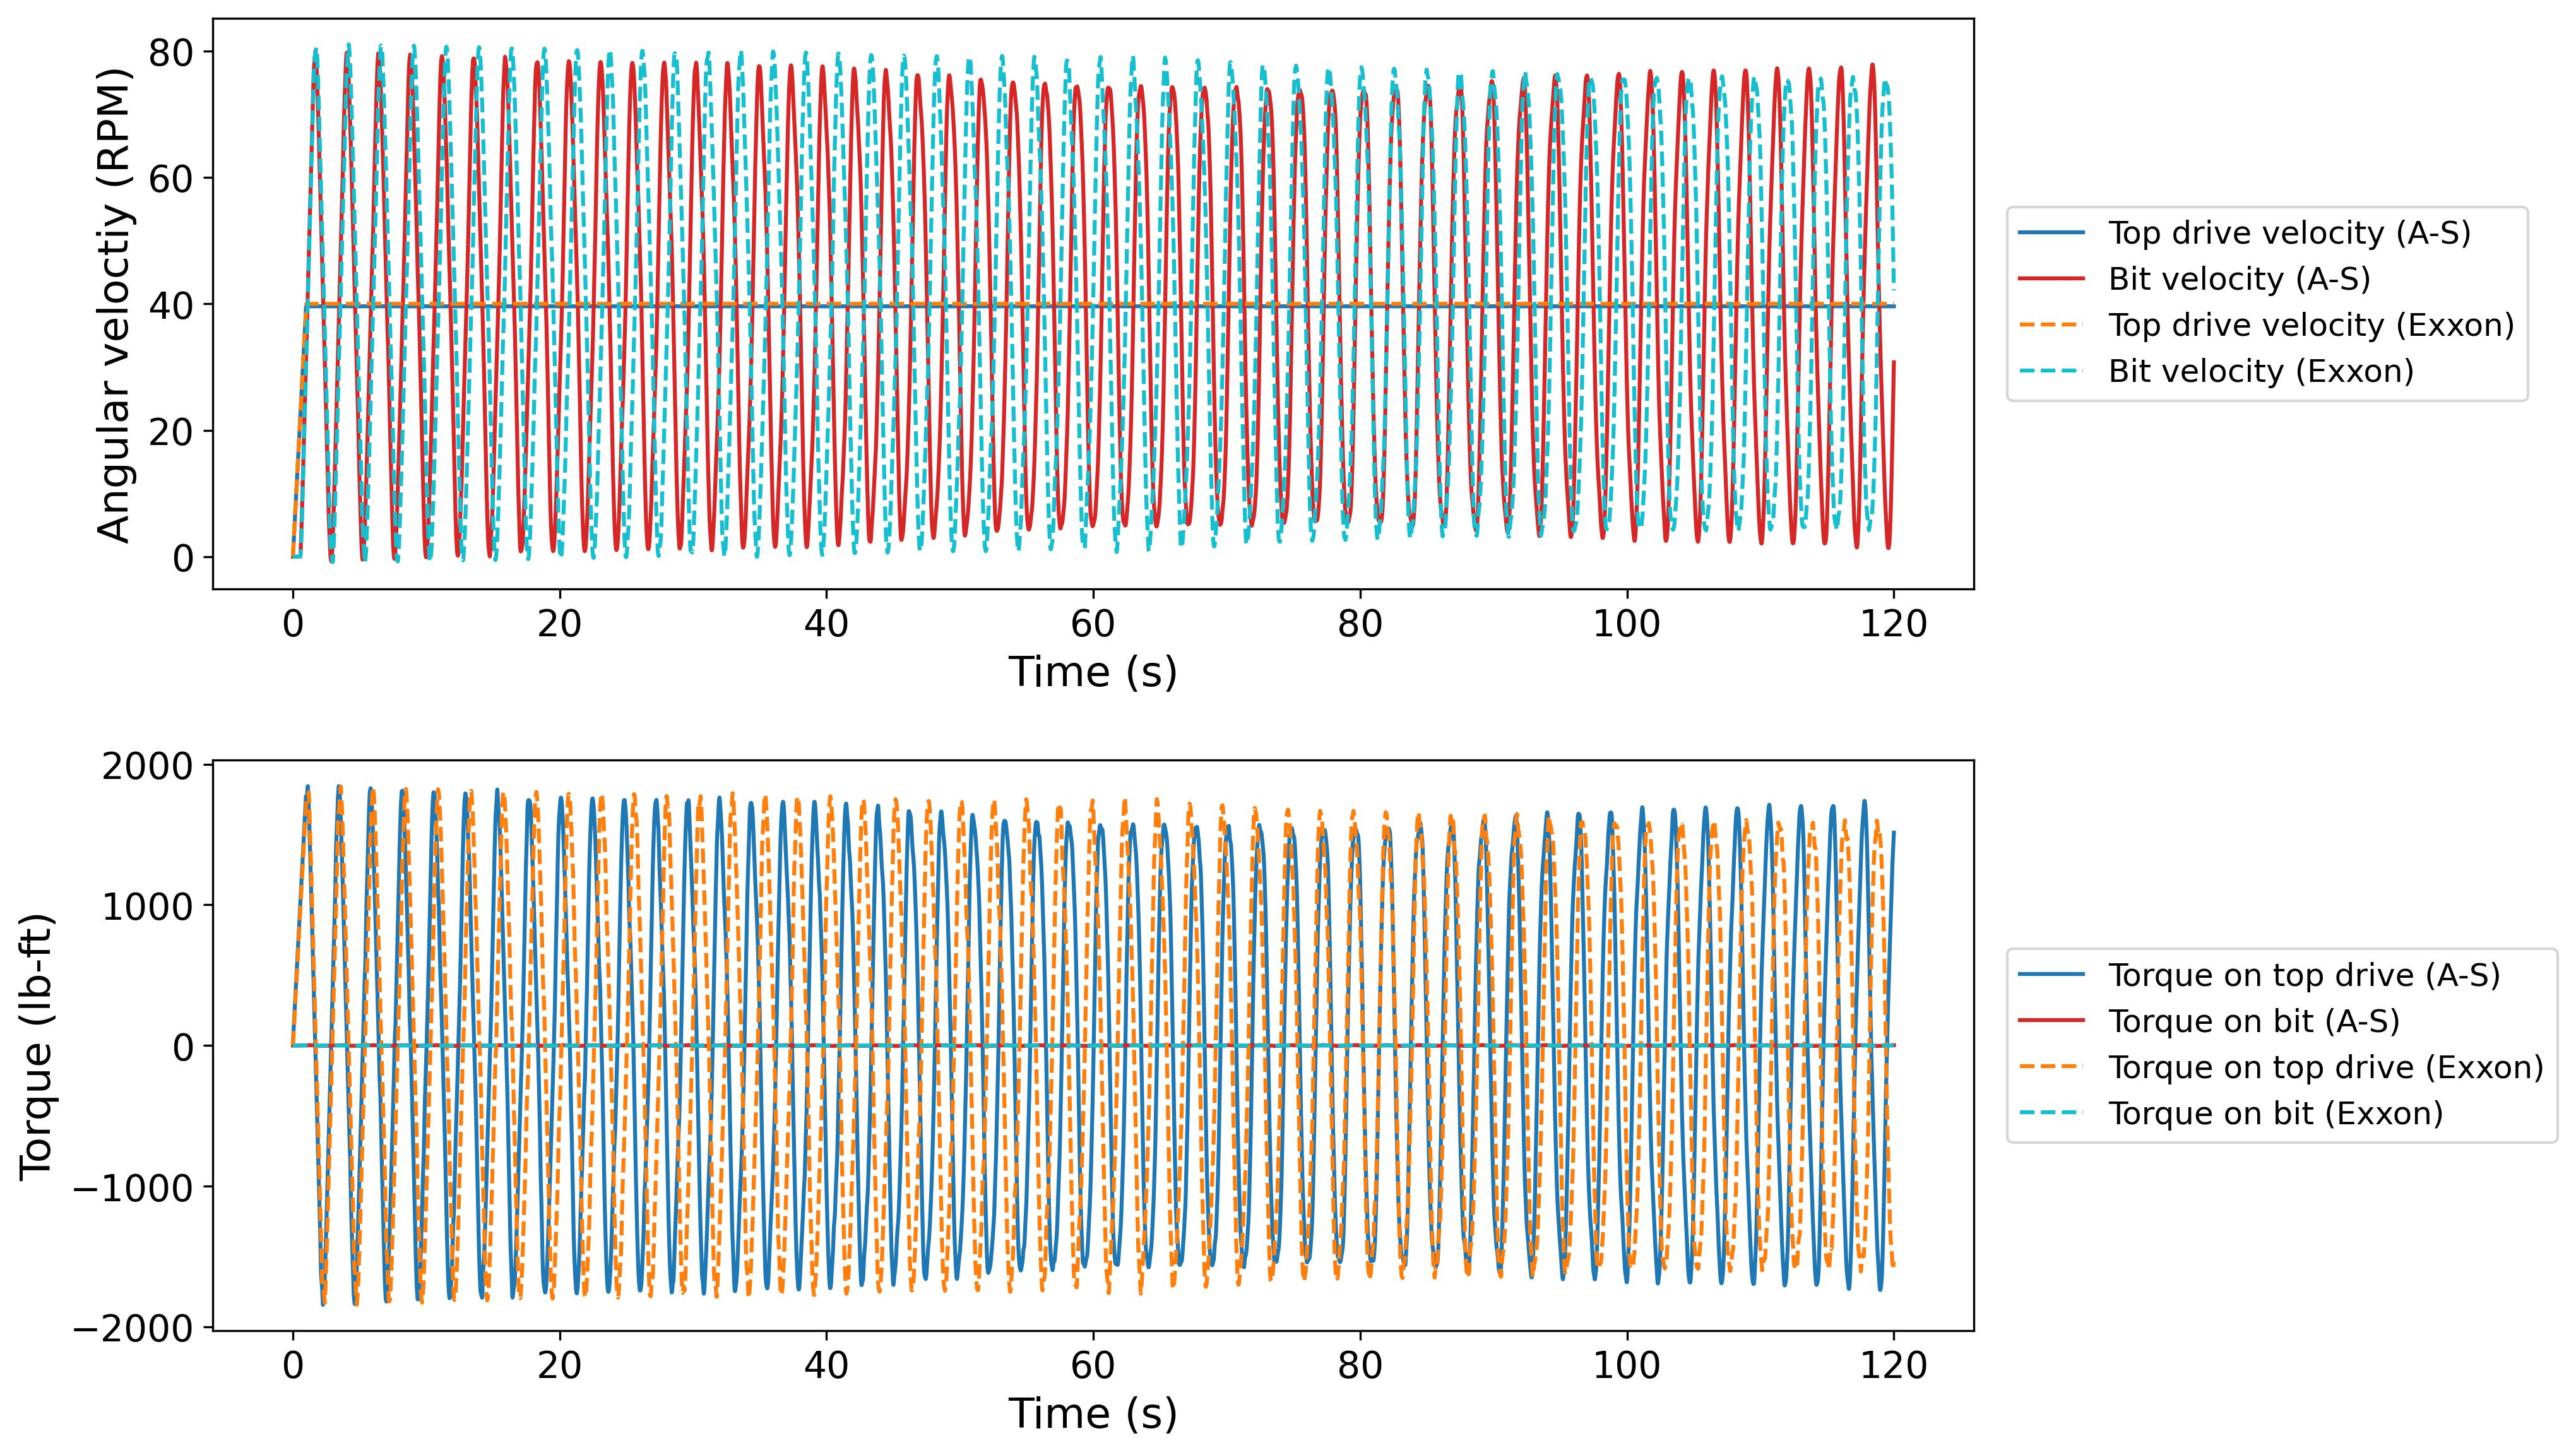
\includegraphics[width=6.5in]{overlapped_figureTestCase3_1}
  \caption[Comparison of the results for Test Case 3]{Comparison between the results from A-S model (MATLAB ver.) and ExxonMobil model for Test Case 3. The fundamental vibration frequency are 0.280 from A-S model and 0.269 from ExxonMobil model. The difference in frequency is small, but the accumulated effect of these differences caused the phase shift during 60 seconds. Overall, both models matched well. The fluctuations of the amplitude of bit angular velocity and top drive torque are observed, which results from BHA components.}\label{figure_testcase3_overlapped}
\end{figure}

\section{Test Case 4}
Results for Test Case 4a for each model and the comparison between the two models are depicted in \figurename~\ref{figure_testcase4_1}, and \ref{figure_testCase4_1_overlapped}. Compared to the difference between Test Case 1 and 3 (BHA effect on vertical well), The effect of BHA components were more significant when comparing Test Case 2a and 4a. The maximum top drive torque increased for about 1500 lb-ft when adding the BHA components to the drill string, while the bit angular velocity was almost the same. This increased effect of the BHA components in Test Case 2a and 4a, compared to Test Case 1 and 3, can be the results of increased depth, Coulomb friction, and decreased shear modulus (refer to input parameters in \chaptername~\ref{ch:testcases}). Additional sensitivity tests can be conducted to analyze the effect of BHA components on drill string vibration.

\begin{figure}
  \centering
  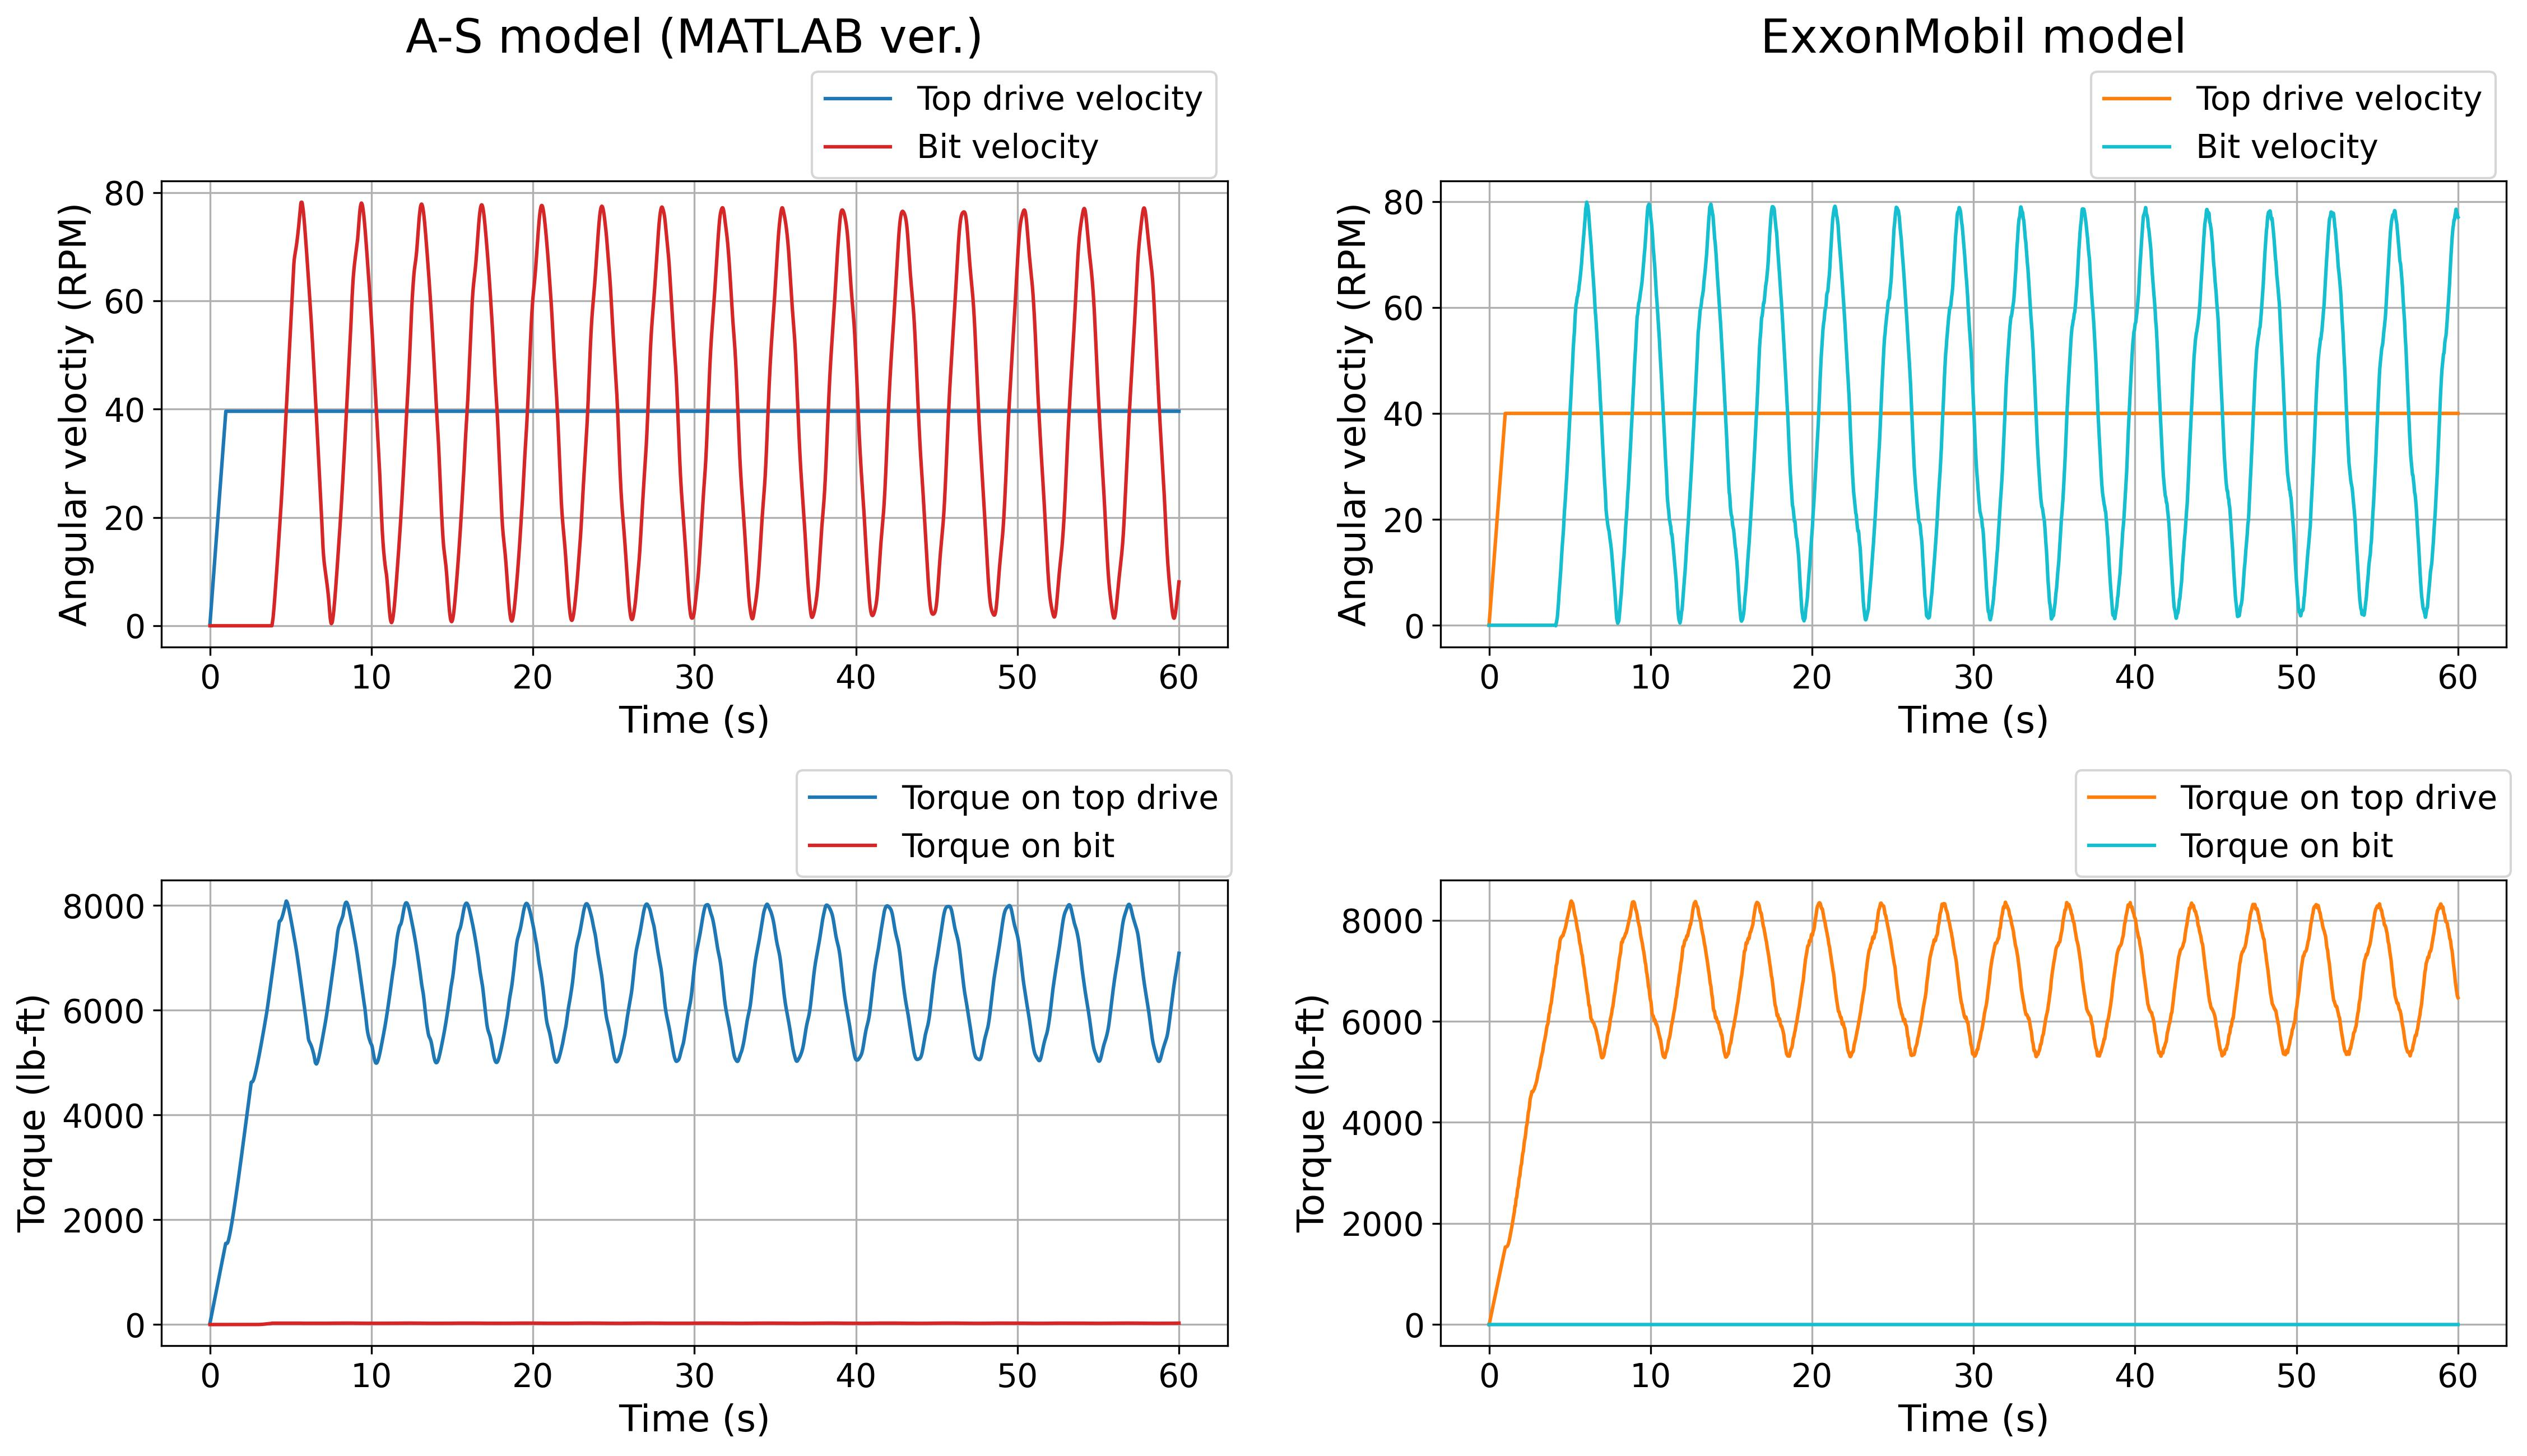
\includegraphics[width=6.5in]{output_figureTestCase4_1}
  \caption[Results of Test Case 4a]{Results of Test Case 4a. First and second columns show the results from A-S model (MATLAB ver.) and ExxonMobil model, respectively.}\label{figure_testcase4_1}
\end{figure}

\begin{figure}
  \centering
  \includegraphics[width=6.5in]{overlapped_figureTestcase4_1}
  \caption[Comparison of the results for Test Case 4a]{Comparison between the results from A-S model (MATLAB ver.) and ExxonMobil model for Test Case 4a. The fundamental vibration frequency are 0.268 from A-S model and 0.260 from ExxonMobil model. The difference in frequency is small, but the accumulated effect of these differences caused the phase shift during 60 seconds. Overall, both models matched well.}\label{figure_testCase4_1_overlapped}
\end{figure}


\subsection{Test Case 4b}
The comparison between A-S, and ExxonMobil model are illustrated in \figurename~\ref{figure_testcase4_2_overlapped}. Both models matched the overall behavior of stick-slip event except the shift in the phase during 60 seconds modeling. The effect of BHA components in deviated well is more detailed in \figurename~\ref{figure_BHA_EXXON}, and \ref{figure_BHA_MATLAB} from ExxonMobil, and A-S model, respectively. Adding the BHA slowed down the vibration while increased the torque on top drive. Specifically, the spikes on top drive were observed in both models before the stick phase. These sudden spikes were more significant in A-S model.


\begin{figure}
  \centering
  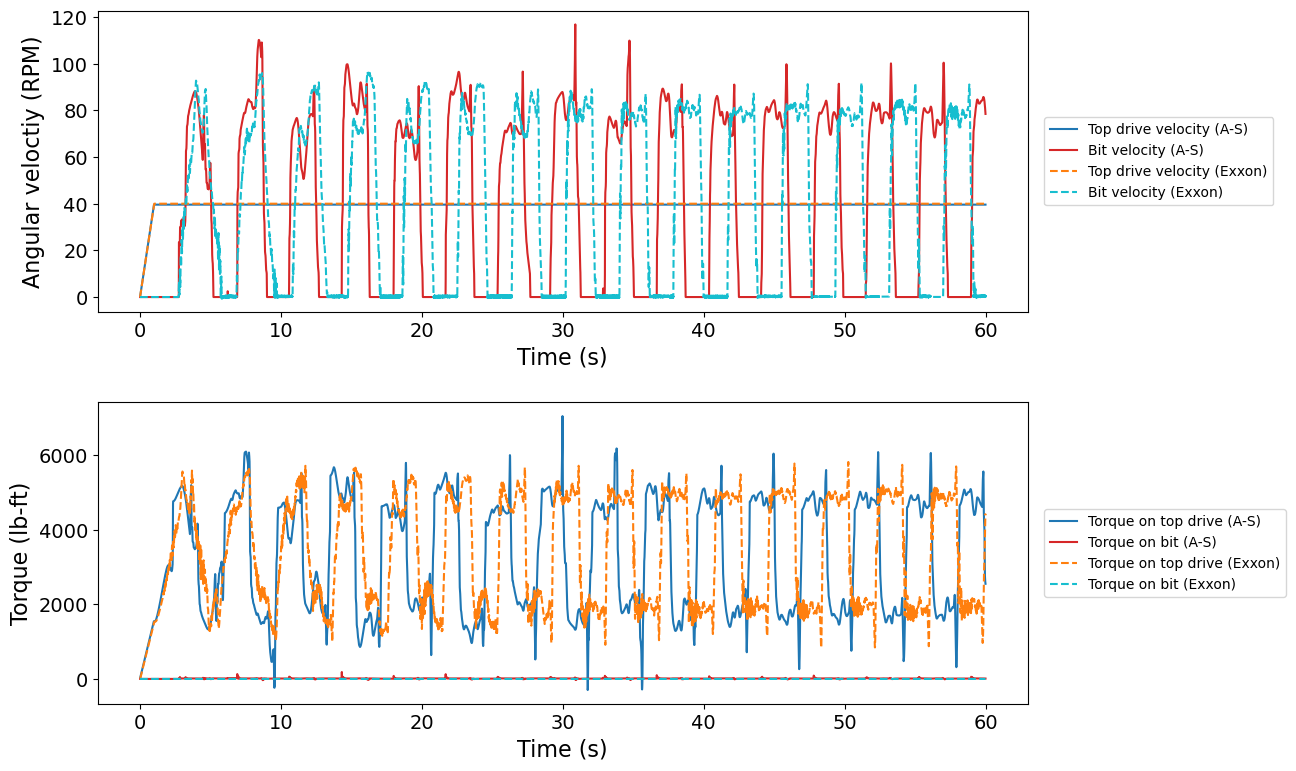
\includegraphics[width=6.5in]{overlapped_figureTestCase4_2}
  \caption[Comparison of the results for Test Case 4b]{Comparison between the results from A-S model (MATLAB ver.) and ExxonMobil model for Test Case 4b. The fundamental vibration frequency are 0.268 from A-S model and 0.260 from ExxonMobil model. The difference in frequency is small, but the accumulated effect of these differences caused the phase shift during 60 seconds. Overall, both models matched well. Especially the transient phase (before 40s) showed similar vibration patterns for both models. Both models predicted a similar stick time of about 1.6-1.7 seconds during the steady phase (after 40s). The spikes in bit angular velocity and torque on top drive were observed from both models, which was not observed when there was no BHA. The amount of spike is more significant in A-S model compared to ExxonMobil model.}\label{figure_testcase4_2_overlapped}
\end{figure}

\begin{figure}
  \centering
  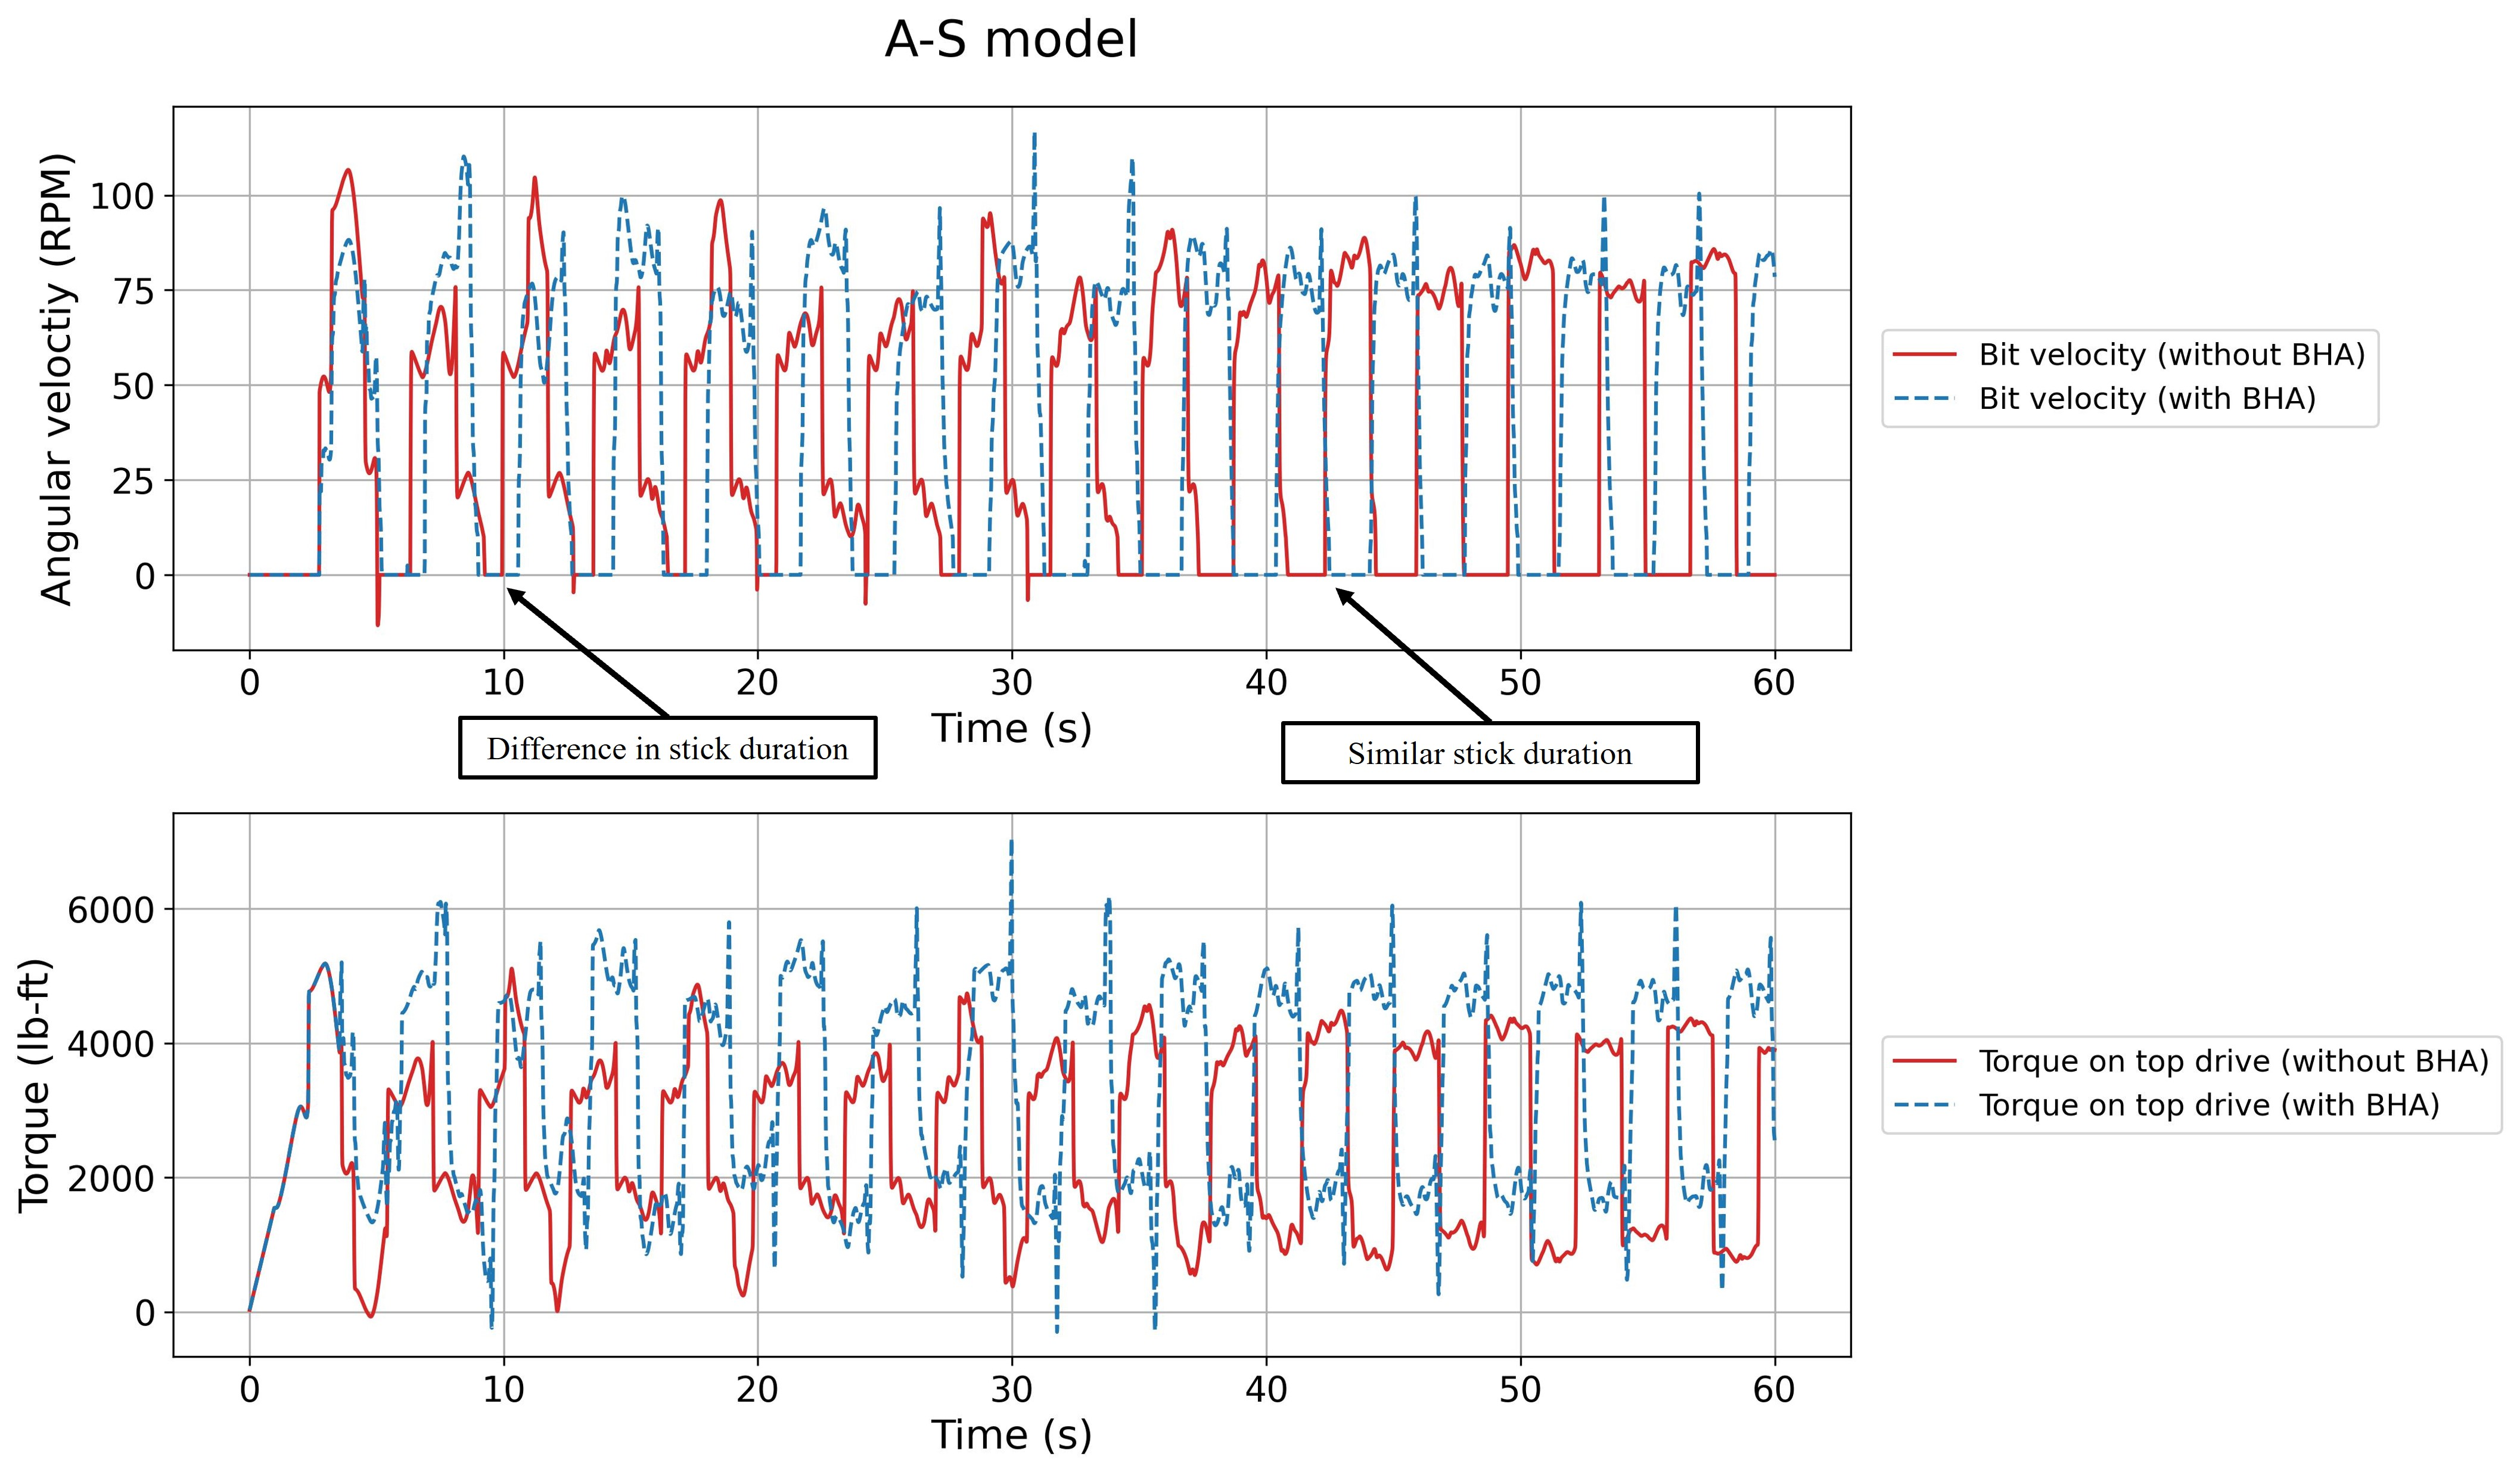
\includegraphics[width=6.5in]{BHA_ml_arrow}
  \caption[Effects of BHA components (MATLAB model)]{Effects of BHA components in deviated wells in A-S model. The graph shows the comparison between Test Case 2b and 4b. Adding BHA components increased torque on top drive while rotating the bit at a similar velocity. The spikes in torque and bit velocity are observed when BHA is added. On the other hand, spikes below 0 RPM on bit velocity are only observed when there are no BHA components. The period of stick-phase is longer for about 2-3 cycles from the beginning when BHA exists; however, it becomes similar which is about 1.6-1.8 s. The fundamental frequency of the vibration decreases when BHA exists.}\label{figure_BHA_MATLAB}
\end{figure}

\begin{figure}
  \centering
  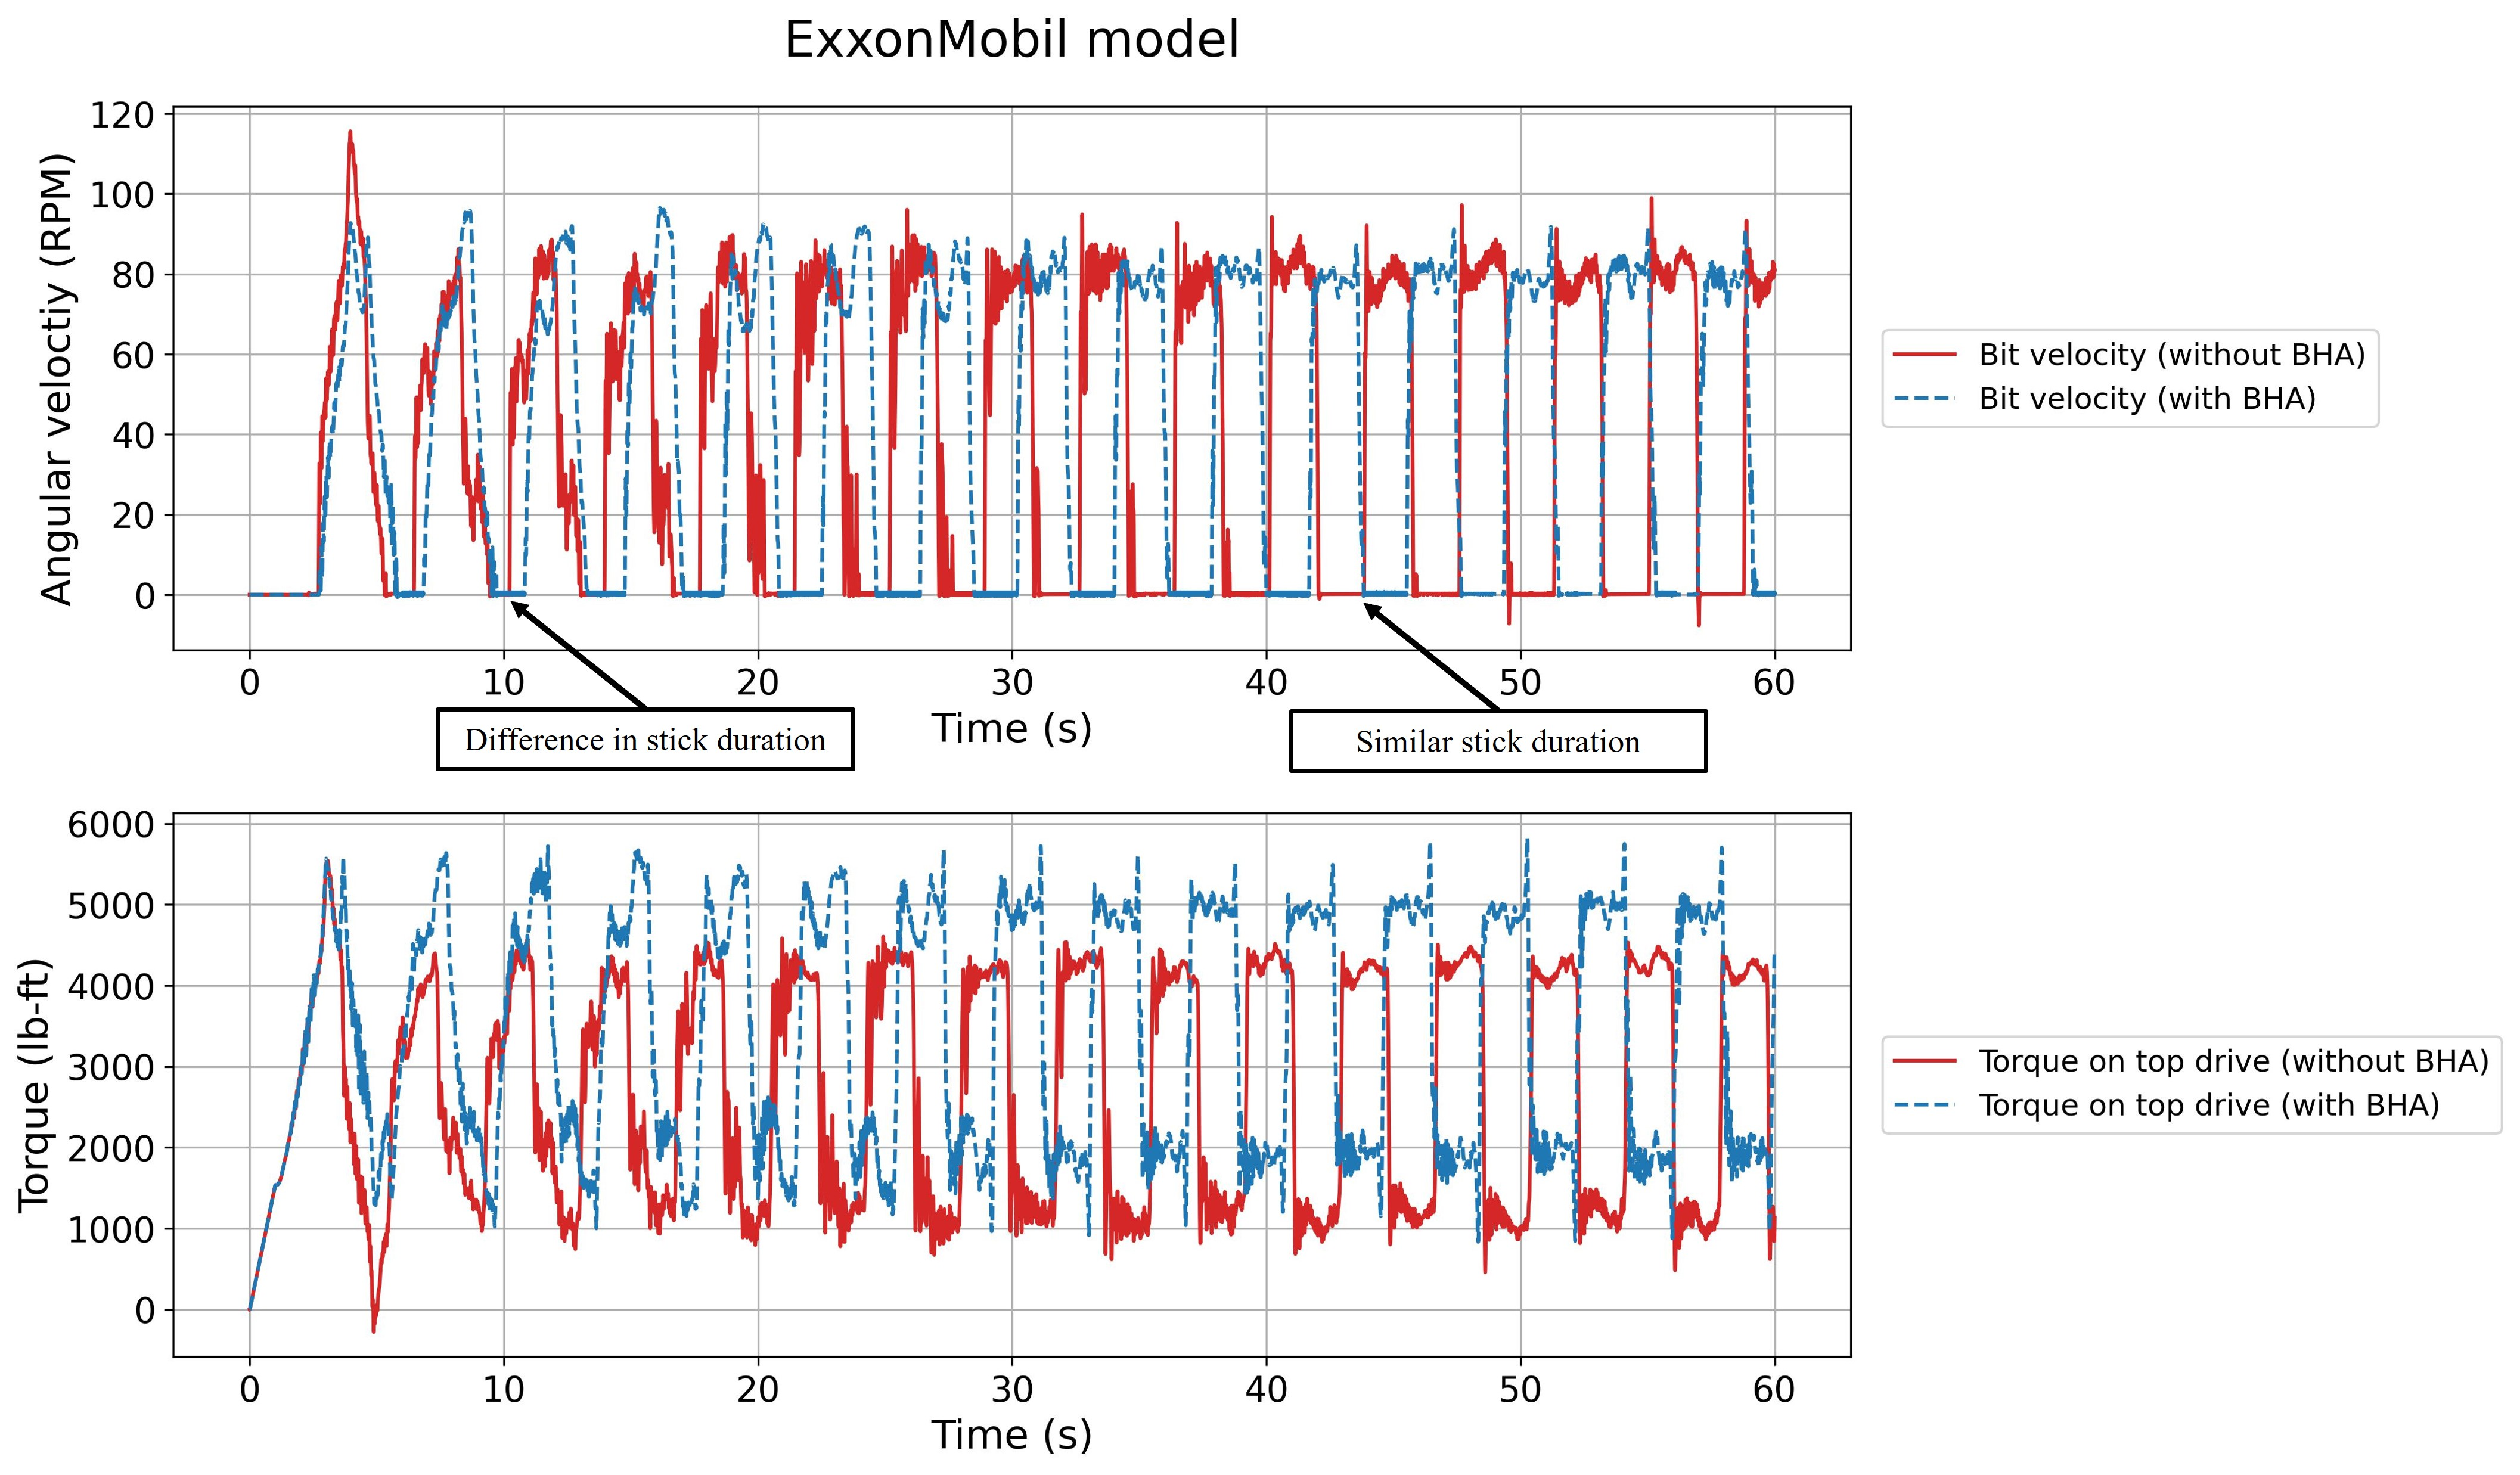
\includegraphics[width=6.5in]{BHA_exxon_arrow}
  \caption[Effects of BHA components (ExxonMobil model)]{Effects of BHA components in deviated wells in ExxonMobil model. The graph shows the comparison between Test Case 2b and 4b. Adding BHA components increased torque on top drive while rotating the bit at a similar velocity. The spikes in torque and bit velocity are observed when BHA is added. On the other hand, spikes below 0 RPM on bit velocity are only observed when there are no BHA components. The period of stick-phase is longer for about 2-3 cycles from the beginning when BHA exists; however, it becomes similar which is about 1.6-1.8 s. The fundamental frequency of the vibration decreases when BHA exists.}\label{figure_BHA_EXXON}
\end{figure}


\section{Summary} 
\begin{table}
    \centering
    \begin{tabular}{|c|c|c|c|c|c|c|}
        \hline
        \textbf{Test Cases} & \textbf{Frequency (Hz)} & \textbf{Max top drive torque (lb-ft)} & \textbf{Max bit velocity (RPM)}\\
        \hline
        Test Case 1 & 0.440 & 1762 & 79\\
        \hline
        Test Case 2a & 0.283 & 6643 & 78\\
        \hline
        Test Case 2b & 0.280 & 5184 & 106\\ 
        \hline
        Test Case 3 & 0.420 & 1844 & 80 \\                                                  
        \hline
        Test Case 4a & 0.268 & 8083 & 78 \\                                                   
        \hline
        Test Case 4b & 0.268 & 7056 & 116\\                                                       
        \hline
    \end{tabular}
    \caption[Input parameters of Aarsnes-Shor model (Python ver.)]{Input parameters of Aarsnes-Shor model. Well trajectory, top drive set velocity, and bit constant are the additional parameters not included in this table.}
    \label{AS_results_summary}
\end{table} 

\begin{table}
    \centering
    \begin{tabular}{|c|c|c|c|c|c|c|}
        \hline
        \textbf{Test Cases} & \textbf{Frequency (Hz)} & \textbf{Max top drive torque (lb-ft)} & \textbf{Max bit velocity (RPM)}\\
        \hline
        Test Case 1  & 0.427 & 1814 & 81\\
        \hline
        Test Case 2a  & 0.272 & 6891 & 79\\
        \hline
        Test Case 2b  & 0.269 & 5539 & 115\\ 
        \hline
        Test Case 3  & 0.408 & 1841 & 81\\                                                  
        \hline
        Test Case 4a  & 0.260 & 8379 & 79\\                                                   
        \hline
        Test Case 4b & 0.260 & 5825 & 96\\                                                       
        \hline
    \end{tabular}
    \caption[Input parameters of Aarsnes-Shor model (Python ver.)]{Input parameters of Aarsnes-Shor model. Well trajectory, top drive set velocity, and bit constant are the additional parameters not included in this table.}
    \label{Exxon_results_summary}
\end{table}

\section{Conclusion}
The availability of these well-structured Test Cases allows for rigorous comparison and verification of drill string models, enabling researchers and engineers to assess their accuracy and performance in various wellbore scenarios. The data and findings obtained from these Test Cases offer valuable insights and constitute a substantial contribution to the field of drill string modeling and simulation. As a result, this study serves as a valuable reference for further research and development in the domain of drilling engineering and related disciplines. 